\documentclass[journal]{IEEEtran}

\usepackage{listings}
\usepackage{xcolor}
\usepackage{graphicx}
\usepackage{amsmath}
\usepackage{amssymb}
\usepackage{booktabs}
\usepackage{caption}
\usepackage{subcaption}
\usepackage{bm}
\usepackage{titlesec}
\usepackage[hidelinks]{hyperref}
\usepackage{floatrow}
\usepackage{blindtext}
\usepackage{cases}
\usepackage{svg}
\usepackage{graphicx}
\usepackage{url}
\usepackage[linesnumbered]{algorithm2e}
\usepackage{algpseudocode}

\renewcommand{\algorithmiccomment}[1]{\bgroup\hfill//~#1\egroup}

\definecolor{codegreen}{rgb}{0,0.6,0}
\definecolor{codegray}{rgb}{0.5,0.5,0.5}
\definecolor{codepurple}{rgb}{0.58,0,0.82}
\definecolor{backcolour}{rgb}{0.95,0.95,0.92}

\lstdefinestyle{mystyle}{
    backgroundcolor=\color{backcolour},   
    commentstyle=\color{codegreen},
    keywordstyle=\color{magenta},
    numberstyle=\tiny\color{codegray},
    stringstyle=\color{codepurple},
    basicstyle=\ttfamily\footnotesize,
    breakatwhitespace=false,         
    breaklines=true,                 
    captionpos=b,                    
    keepspaces=true,                 
    numbers=left,                    
    numbersep=5pt,                  
    showspaces=false,                
    showstringspaces=false,
    showtabs=false,                  
    tabsize=2
}

\lstset{style=mystyle}

\hyphenation{op-tical net-works semi-conduc-tor}

\begin{document}

% paper title
\title{Offboard drone application using different positioning techniques}

% author names and IEEE memberships
\author{Giacomo Corradini,~\IEEEmembership{Student ID number 236873},  \\
Mattia Pettene,~\IEEEmembership{Student ID number 239145}
        }% <-this % stops a space

% make the title area
\maketitle

% As a general rule, do not put math, special symbols or citations
% in the abstract or keywords.
\begin{abstract}
This report, in the domain of Unmanned Aerial Vehicles, investigates the efficacy of three drone positioning methods: Global Positioning System (GPS), Motion Capture (MoCap), and Ultra WideBand (UWB), implemented within the PX4 and ROS2 environment. The primary objective is to evaluate their performance, highlighting respective strengths and challenges during an offboard application. In the entirety of the project, a structured two-phase methodology was adopted, starting from simulations succeeded by empirical real-world trials for practical validation. The results demonstrate commendable precision and reliability using the MoCap method, while GNSS proved effective but makes it more difficult to control the drone in position. Instead the UWB approach, while promising in simulation, necessitates refinement due to significant interference and noise in a real environment, affecting its accuracy. 
\vspace{3mm}

Index Terms -- Unmanned Aerial Vehicles (UAVs), Global Navigation Satellite Systems (GNSS), Global Positioning System (GPS), Motion Capture (MoCap), Ultra-WideBand (UWB), differential time difference of arrival (DTDOA). 

\end{abstract}

\IEEEpeerreviewmaketitle

\section{Introduction}

The use of drones, also known as Unmanned Aerial Vehicles (UAVs), has revolutionized the landscapes of applications, both outdoors and indoors, introducing new perspectives and possibilities across a wide range of fields. The ability to collect real-time data, execute specific missions, and reach inaccessible or confined locations has made drones a valuable resource for various industries and sectors. Outdoors, UAVs have become essential tools for precision agriculture, infrastructure inspection, topographic mapping, environmental surveillance, and even emergency response. At the same time, the use of drones indoors has opened up new horizons in logistics, industrial automation, and security. 

This report aims to analyze three different positioning methods to be used in these real applications, both outdoor (GPS) and indoor (MoCap and UWB). Global Positioning System (GPS) is a widely used satellite-based positioning method for navigation and localisation in outdoor contexts, Motion Capture (MoCap) is a system relying on cameras that track the drone's movement using reference points in the surrounding environment and Ultra-WideBand (UWB) is a technology based on transmitting ultra-wideband signals to determine relative positions in indoor situations. 

The analysis was conducted by performing a simple autonomous flight, using the ROS2 (Robot Operating System 2) framework in conjunction with the PX4 platform, which provides a versatile and highly configurable development and testing environment. 

The decision to employ the PX4 platform was motivated by its collaborative support and flexibility shown in some research based on the same architecture\cite{montemurro} \cite{malacarne}, its configurability to suit specific project needs, and its reliability in offering interfaces for sensor integration.

Additionally, an analysis of UWB as a positioning method conducted in another work \cite{conte} demonstrated promising outcomes, leading to consider UWB as a viable positioning method. 
In particular, \cite{conte} utilises UWB to enhance positioning in indoor environments, where GNSS signals are unavailable. The system employs a combination of sensor fusion algorithms, including Kalman filters, to obtain a reliable pose estimation and it is validated in both simulation and real-world experiments, demonstrating its effectiveness in achieving similar results in both GNSS-enabled and denied environments. Moreover, \cite{vicon} proposes a new 3D velocity estimation solution based on Ultra WideBand signals for navigation of UAVs in indoor environments. The authors implemented linear Kalman filters for removing noise on the range measurements and the vertical position estimate. The solution is verified with three experimental scenarios with manual and autonomous flights of a quadrotor, using a motion capture system as ground truth. A relatively inexpensive solution for both position and velocity estimation is achieved using the UWB system, with sufficient accuracy for autonomous flight of UAVs in indoor areas. 

The main contributions of this work can be summarised as follows: 
\begin{itemize}
    \item provide a comprehensive and detailed overview of the performance of the different positioning systems tested while performing an autonomous flight;
    \item identify advantages, limitations, and optimal use scenarios for each technique to provide useful guidance for future developments and practical applications in the field of drones.
\end{itemize}

The rest of the report is organised in the following way. Sections \ref{px4_overview} and \ref{px4_arch_overview} reported an overview of PX4 architecture on which this work is based, while in Section \ref{pos_tech} are described in a theoretical way the three positioning methods analysed. The hardware used to carry out this study, such as the drone and the environment setup is explained in Section \ref{hardware}. Finally, simulations and experimental results are reported respectively in Section \ref{simulations} and Section \ref{experimental}.

All project-related materials, including the code and detailed installation guides for PX4 and ROS2, as well as instructions on running the simulations, are available on the dedicated GitHub repository \cite{git}.

\section{PX4 overview}
\label{px4_overview}
"PX4 is the Professional Autopilot. Developed by world-class developers from industry and academia, and supported by an active worldwide community, it powers all kinds of vehicles from racing and cargo drones through to ground vehicles and submersibles" \cite{PX4_paper}.

Its main properties are:

\begin{itemize}
    \item Modular Architecture
    \item Open-source
    \item Robust and deep integration with companion computers and robotics APIs (ROS 2, MAVSDK).
\end{itemize}

\subsection{High-level overview}

The PX4 configurations used for offboard applications (the studied one) include both a flight controller and a companion computer (Fig. \ref{fig:px4_general_architecture}) (also known as a "mission computer") \cite{px4_architecture}.

\begin{figure}
    \centering
    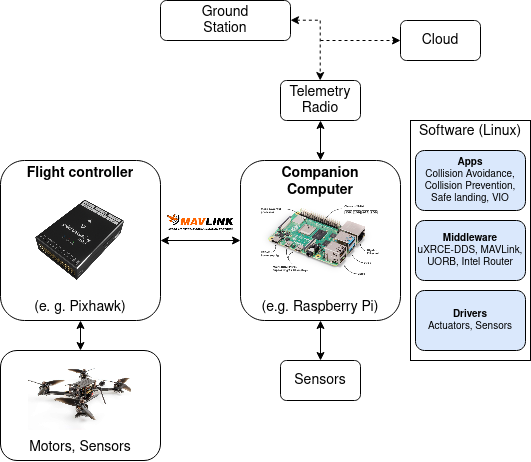
\includegraphics[scale=0.4]{Images/px4_general_architecture.png}
    \caption{Flight Controller and Companion Computer}
    \label{fig:px4_general_architecture}
\end{figure}

The flight controller runs the normal PX4 flight stack, while a companion computer provides advanced features like object avoidance and collision prevention, which allow it to perform offboard applications.

The hardware consists of

\begin{itemize}
    \item Flight controller
    \item Motor ESCs connected to PWM outputs, DroneCAN
    \item Sensors connected via I2C, SPI, CAN, UART etc
    \item Camera or other payload. Cameras can be connected to PWM outputs or via MAVLink
    \item Telemetry radios for connecting to a ground station computer/software
\end{itemize}

\section{PX4 architectural overview}
\label{px4_arch_overview}
"PX4 consists of two main layers: the flight stack is an estimation and flight control system, and the middleware is a general robotics layer that can support any type of autonomous robot, providing internal/external communications and hardware integration" \cite{px4_architecture_flight_stack}.

\subsection{Flight stack architecture}

According to the developer guide, “the flight stack is a collection of guidance, navigation and control algorithms for autonomous drones. It includes controllers for fixed-wing, multirotor and VTOL airframes as well as estimators for attitude and position” \cite{px4_architecture_flight_stack}.

Fig. \ref{fig:px4_flight_stack} shows the connections of the building blocks of the flight stack. It contains the full pipeline from sensors, RC input and autonomous flight control (Navigator), down to the motor or servo control (Actuators):

\begin{figure}
    \centering
    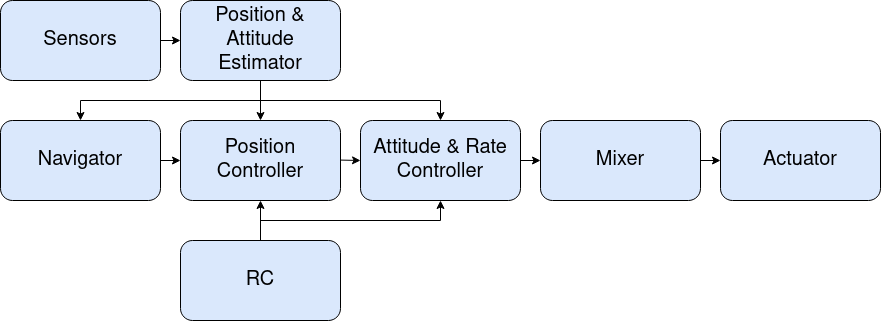
\includegraphics[scale=0.27]{Images/flight_stack.png}
    \caption{Flight stack architecture}
    \label{fig:px4_flight_stack}
\end{figure}

\begin{itemize}
    \item An estimator takes one or more sensor inputs, combines them, and computes a vehicle state (for example the attitude from IMU sensor data).
    \item A controller is a component that takes a setpoint and a measurement or estimated state (process variable) as input. Its goal is to adjust the value of the process variable such that it matches the setpoint. The output is a correction to eventually reach that setpoint.
    \item A mixer takes high-level commands and translates them into individual motor commands, while ensuring that some limits are not exceeded. This translation is specific for each vehicle type.
\end{itemize}

\subsection{Control stack}

The control stack is the part of the system that allows the drone to fly, its correctness depends mostly on the correct estimation of the drone’s state.

In Fig. \ref{fig:mc_control_arch} it is possible to acknowledge the capabilities of the controller, which is able to allow multiple sources of control for the user. The positioning control is the most complex and requires a complete knowledge of the feedback for all the blocks in the control stack: position, velocity, acceleration, attitude and angular rate.

% This work focuses on giving the correct feedback to the control stack in any situation, even in a GNSS denied scenario, and then it lets the stack deal with the actuation of the rotors to reach correct and stable positioning.

\begin{figure}
    \centering
    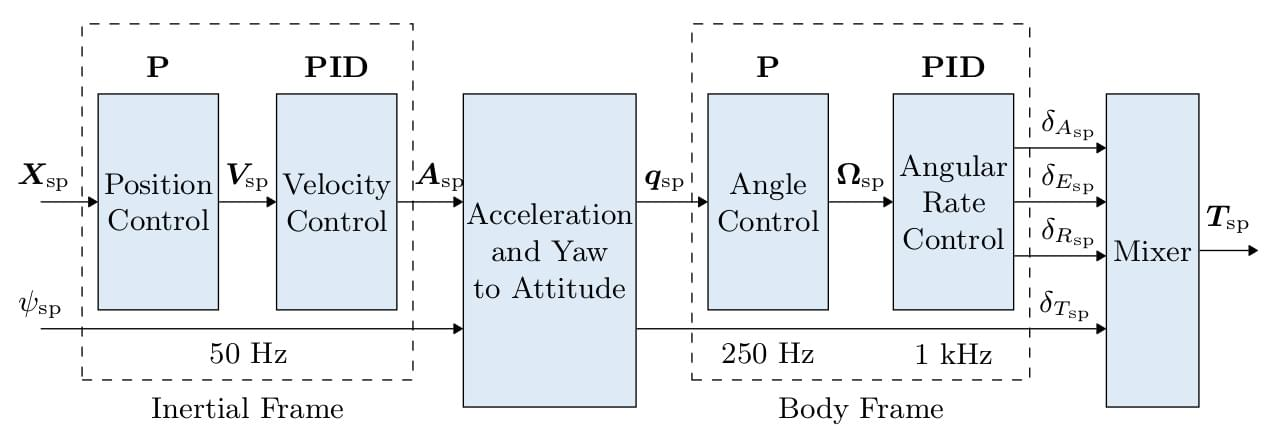
\includegraphics[scale=0.19]{Images/mc_control_arch.jpg}
    \caption{Control stack}
    \label{fig:mc_control_arch}
\end{figure}

\subsection{Middleware}

"The middleware consists primarily of device drivers for embedded sensors, communication with the external world (companion computer, GCS, etc.) and the uORB publish-subscribe message bus" \cite{px4_architecture_flight_stack}.

\textbf{uORB} is an asynchronous publish() / subscribe() messaging API used for inter-thread/inter-process communication. 

"PX4 uses \textbf{uXRCE-DDS middleware} to allow uORB messages to be published and subscribed on a companion computer as though they were ROS2 topics. This provides a fast and reliable integration between PX4 and ROS2, and makes it much easier for ROS2 applications to get vehicle information and send commands" \cite{px4_middleware}.

\begin{figure}
    \centering
    \includesvg[scale=0.35]{Images/architecture_xrce-dds_ros2}
    \caption{uXRCE-DDS architecture}
    \label{fig:uXRCE-DDS}
\end{figure}

In Fig. \ref{fig:uXRCE-DDS} is shown the uXRCE-DDS architecture. The uXRCE-DDS middleware consists of a client running on PX4 and an agent running on the companion computer, with bi-directional data exchange between them over a serial or UDP link. The agent acts as a proxy for the client, enabling it to publish and subscribe to topics in the global DDS data space.

\subsection{Commander}

The commander is the central block for PX4 architecture, basically the PX4 brain, it takes inputs from sensors, estimators, QGC, RC controller; then based on the vehicle condition and the command received by the user it sets the “vehicle control mode”, it also handles flight failure (fail-safe strategies). 

The commander module subscribes to a huge number of topics as can be seen in Fig. \ref{fig:uorb_graph}.

\begin{figure}
    \centering
    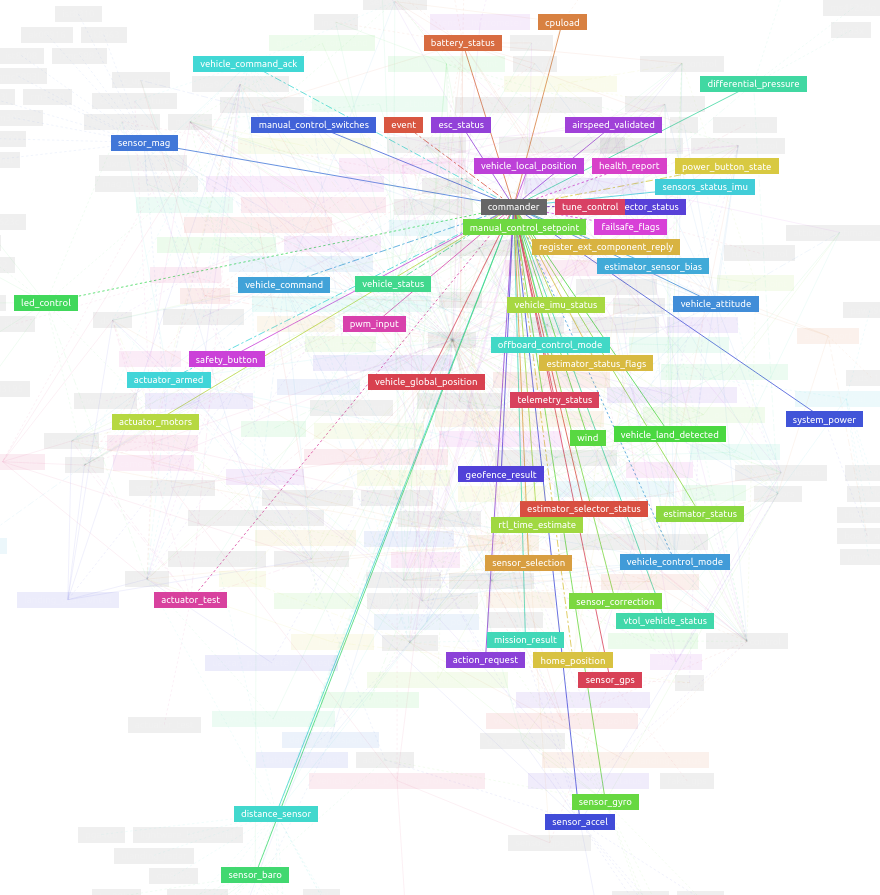
\includegraphics[scale=0.25]{Images/uorb_graph.png}
    \caption{Commander Topics}
    \label{fig:uorb_graph}
\end{figure}

Thus, publishing control commands to the commander module topics makes it possible to control the vehicle.

\section{Positioning techniques}
\label{pos_tech}
\subsection{Global Navigation Satellite System}

"Global Navigation Satellite Systems include constellations of Earth-orbiting satellites that broadcast their locations in space and time, of networks of ground control stations, and of receivers that calculate ground positions by trilateration" \cite{gnss}.

Different systems are actually fully functional:

\begin{itemize}
    \item Global Positioning System (GPS)
    \item GLObal NAvigation Satellite System (GLONASS)
    \item European Satellite Navigation System (GALILEO)
    \item COMPASS/Bei-Dou
    \item Regional Navigation Satellite System (IRNSS)
    \item Quasi-Zenith Satellite System (QZSS)
\end{itemize}

Once all these global and regional systems become fully operational, the user will have access to positioning, navigation and timing signals from more than 100 satellites \cite{gnss}.

A GNSS is also composed of ground stations to monitor and control the satellite's orbit and provide necessary corrections and manoeuvring. Fig \ref{gnss_figure} represents the connection between the space segment composed by the satellites, the ground segment that controls them and a GNSS equipment mounted on a drone.

\begin{figure}
    \centering
    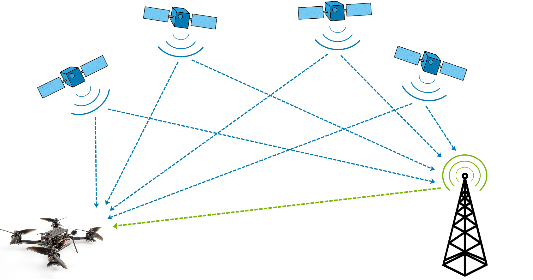
\includegraphics[scale=0.33]{Images/gnss.png}
    \caption{GNSS connection scheme.}
    \label{gnss_figure}
\end{figure}

At least the GNSS user equipment receives the signals from the constellation with a receiver, calculates the ranging data from the antenna to each satellite, and then the navigation processor computes a position, velocity and time solution. Different user equipment have more functionalities with increasing cost: power supply, user interface, the capability to fuse ranging information with other sensors and multiple constellations support.

\subsection{Motion capture} 
Motion capture is the process of recording the movement of objects or people and translating it into data. 

Essentially motion is recorded by tracking the precise position and orientation of points of interest at high frequency. Each tracker uses fundamentally different physical principles to measure position and orientation.

Measurement error is reduced to a minimum with advanced tracking algorithms and post-processing. Several different sensing mechanisms can track sufficient motion leading to a wide variety of uses in autonomous systems \cite{Rahul2018ReviewOM}. 

\subsection{Ultra WideBand}
Ultra WideBand is a radio technology that involves generating and transmitting narrow-duration pulses, resulting in a very wide transmission bandwidth. The main advantages of UWB are the low complexity and cost and the robust interference immunity. Besides this, Ultra WideBand presents high resolution in time and space, obstacle penetration capability and ranging accuracy, which make it ideal for indoor positioning and localisation \cite{uwb_advantages}. In order to use UWB technology as a positioning system it is necessary to define a sensor to be located, called tag, and at least three sensors with known positions, called anchors. There are several algorithms to extract the tag position in UWB-based localisation systems, among which the simplest use geometric methods, such as trilateration and multilateration algorithms \cite{uwb_algorithms}. The second is a generalisation of the first, since it uses $n$ anchors instead of just three, as it is possible to observe in Fig. \ref{fig:sphere}. 

Given an reference anchor $A_0(0,0,0)$ and $n$ generic anchors $A_n(x_n,y_n,z_n)$ the set of equations of multilateration algorithm, that allows to extract the tag position $x$, can be written in matrix form as follows:
\begin{equation}
    Ax = b
    \label{eq:mult}
\end{equation}
\noindent
where, 
\begin{equation*}
    A \ =  \begin{bmatrix}
      x_1 - x_0 & y_1 - y_0 & z_1 - z_0 \\
      x_2 - x_0 & y_2 - y_0 & z_2 - z_0 \\
           ... \\
      x_n - x_0 & y_n - y_0 & z_n - z_0 \\
      
    \end{bmatrix}, \hspace{0.4cm} x \ =  \begin{bmatrix}
        x_t \\ y_t \\ z_t
    \end{bmatrix},
\end{equation*}

\begin{equation*}
        b =  \frac{1}{2} \cdot 
        \begin{bmatrix}
        d_0^2 - d_1^2  + (x_1^2 + y_1^2 + z_1^2) - (x_0^2 + y_0^2 + z_0^2)\\ 
        d_0^2 - d_2^2  + (x_2^2 + y_2^2 + z_2^2) - (x_0^2 + y_0^2 + z_0^2)\\ 
        ... \\
        d_0^2 - d_n^2  + (x_n^2 + y_n^2 + z_n^2) - (x_0^2 + y_0^2 + z_0^2)\\ 
        \end{bmatrix}
\end{equation*} \\
\noindent
while $d_n$ is the distance (range or radius of a sphere) between the coordinates of the $n$th anchor and the tag. The solution of equation \ref{eq:mult} can be achieved using over-determined least square method \cite{uwb_algorithms} as:
\begin{equation}
    x = (A^TA)^{-1}A^Tb
    \label{eq:lstsqr}
\end{equation}

This multilateration algorithm will be tested in simulation, while in real tests will be used a slightly different version (DTDOA).

\begin{figure}
    \centering
    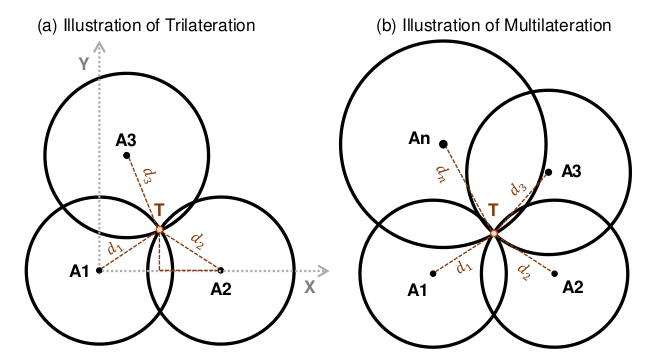
\includegraphics[scale=0.30]{Images/sphere.png}
    \caption{Illustration of trilateration and multilateration algorithm in 2D \cite{uwb_algorithms}.}
    \label{fig:sphere}
\end{figure}

\section{Hardware description}
\label{hardware}
\subsection{Drone setup} \label{Drone-setup}

\begin{figure}
    \centering
    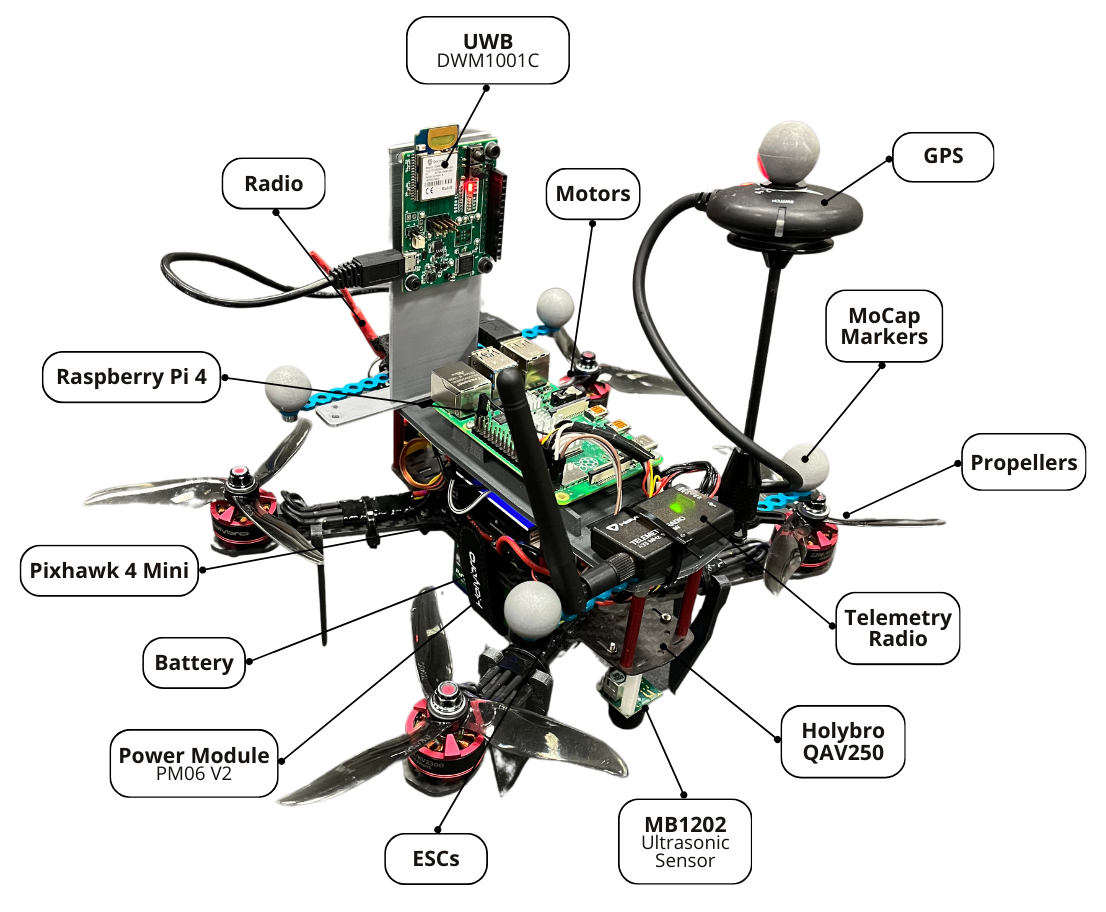
\includegraphics[width=0.9\textwidth]{Images/drone_label.png}
    \caption{Representation of the equipment of the drone.}
    \label{fig:drone}
\end{figure}

To carry out experimental tests, a drone equipped with all the necessary components was used, as it is possible to observe in Fig. \ref{fig:drone}. Starting from an \textbf{Holybro QAV250 Kit} \cite{qav250kit}, that already includes a carbon fiber 250 airframe, motors (2207 KV1950), ESCs (BLHeli S ESC 20A), propellers and a power module (PM06 v2), additional components needed for the different tests were incorporated. 

In particular, one of the most important devices to fly a drone is the flight controller: the mounted one is a \textbf{Pixhawk 4 Mini} \cite{pixhawk4mini}. Pixhawk, which is the reference hardware platform for PX4, is an independent open-hardware project providing readily-available, low-cost, and high-end, autopilot hardware designs to the academic, hobby and industrial communities \cite{pixhawk}. The Pixhawk acts as the central control unit for the vehicle, managing both its flight control and navigation. Using its embedded sensors (accelerometer, gyroscope, barometer and magnetometer) and an external positioning system, it is able to interpret the drone's orientation, velocity, and position in real time. The onboard software processes this information to execute commands, adjust flight parameters, and ensure stable and precise flight control.

Since the project concerns autonomous flight, it is necessary to have an onboard computer that is connected to the flight controller (Fig. \ref{fig:px4_general_architecture}), which enables computationally expensive features like object avoidance and collision prevention. In this project, this function is performed by a \textbf{Raspberry Pi 4 model B} and its main task is that of planning, sending commands to the flight controller in order to follow a desired trajectory. This companion computer runs Ubuntu 22.04 and communicates with the Pixhawk via uXRCE-DDS over a serial port, using the \textit{UART} (Universal Asynchronous Receiver-Transmitter) protocol. 

Given that the project aims to test different positioning systems, the drone has been equipped with specific hardware corresponding to each method being tested. For outdoor flight, a GPS module has been added, connecting it directly to the \textit{GPS MODULE} port of the flight controller. To allow the motion capture system to track the vehicle, markers were mounted on it, as shown in Fig. \ref{fig:drone}. Finally, to use UWB to localise the vehicle, a Decawave DWM1001C module was connected via \textit{USB} to the companion board. In the latter case, since it is not possible to estimate precisely the drone's altitude using this method, an ultrasonic sensor (MaxBotix MB1202) was added to the bottom. The sensor is wired to the Raspberry Pi 4B via \textit{I2C} (Inter-Integrated Circuit) communication.

Lastly, to complete the drone's hardware equipment, a radio receiver and a telemetry radio were mounted: the first allows to take control using a remote control transmitter in case of abnormalities during the autonomous flight, while the second transmits data between the vehicle and a remote control station, such as GPS location, battery status, and other telemetry data. Some custom supports were designed using CAD modelling and then 3D printed.

\subsection{Custom airframe}

In order to achieve a more compact drone, a custom airframe has been realised, by reference to \cite{cinese}. This prototype was designed using CAD modelling and then 3D printed.
The main strength of this customised airframe lies in its adaptability to various applications: it can be configured with either of two companion boards (Raspberry Pi 4 or NVIDIA Jetson Nano) and it is compatible with two distinct flight controllers (Pixhawk 4 mini or Kakute F7). In addition, it is possible to mount an Intel RealSense D430 as a vision system. This prototype is driven by two 18650 batteries as energy supplies. A representation of the drone equipped with the main components is shown in Fig. \ref{fig:cad}. This custom airframe was not employed for the real tests presented in this project, since some specific components were unavailable. However, it can be a powerful tool for future implementations. 

 \begin{figure}
    \centering
    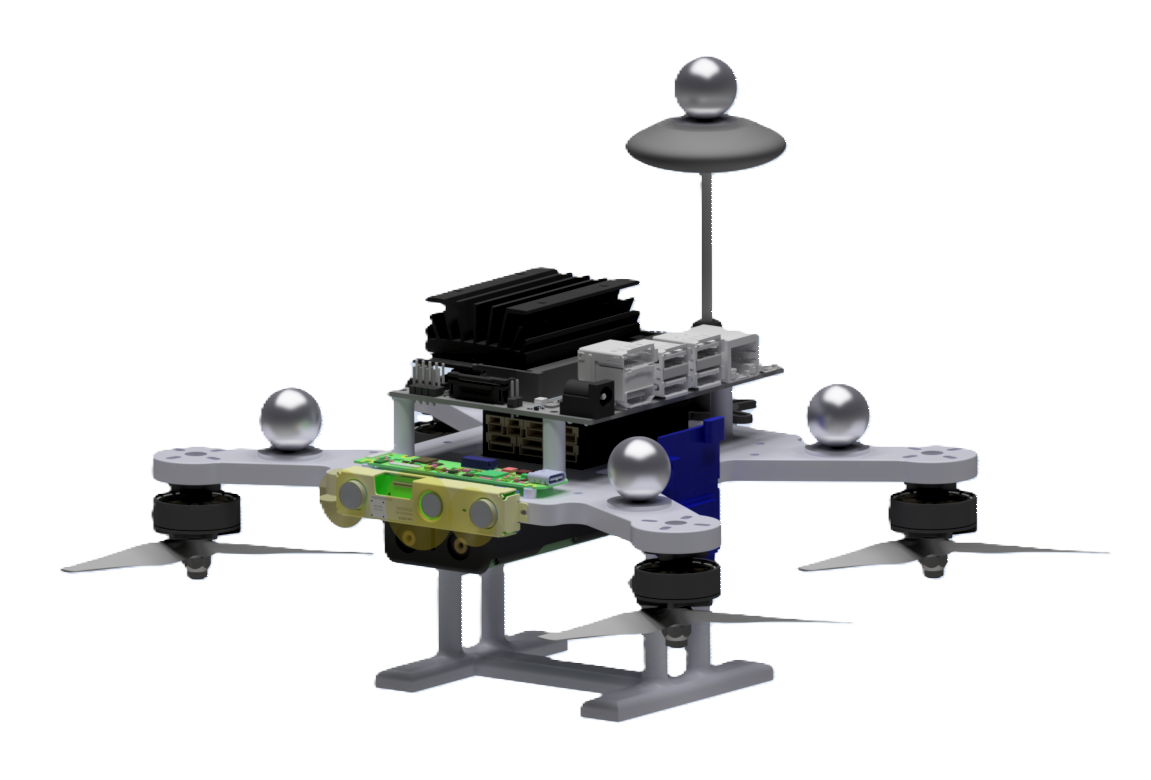
\includegraphics[width=0.9\textwidth]{Images/cad_drone_custom_nosfondo.png}
    \caption{Custom airframe representation.}
    \label{fig:cad}
\end{figure}

\subsection{Environment setup} \label{Environment-setup}

The experimental tests done in this work require two different environmental setups, one for the outdoor tests and one for the indoor ones. 

Regarding the outdoor test only the GPS is needed, is then important to test in a location where the GPS signal is quite good: the parameters to look at to evaluate the goodness of the signal are the number of satellites and the dilution of precision (DOP). This can be easily done using QGroundControl \cite{QGroundControl} and looking at the parameters highlighted in Fig. \ref{fig:QGroundControl}, where the parameters on the top refer to the number of satellites (ideally more than 10) and the parameter on the bottom refer to the dilution of precision (ideally less than 1).

\begin{figure}
    \centering
    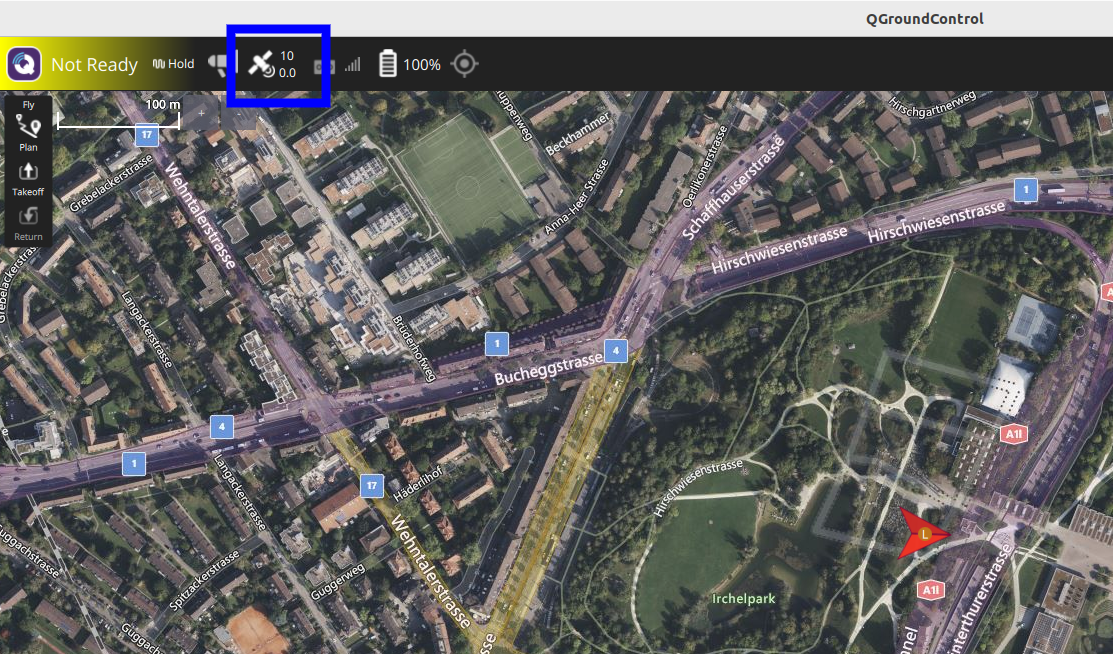
\includegraphics[scale=0.26]{Images/QGroundControl_cut.png}
    \caption{QGroundControl interface}
    \label{fig:QGroundControl}
\end{figure}

For the indoor test, two different infrastructures are used, the motion capture system and the Ultra WideBand system. Fig. \ref{fig:env_hardware} and Fig. \ref{fig:vision_system} represent the environment setup used in this work. Qualysis has been used as a motion capture system and an UWB infrastructure composed of six DWM1001C modules as anchors.

\begin{figure}
    \centering
    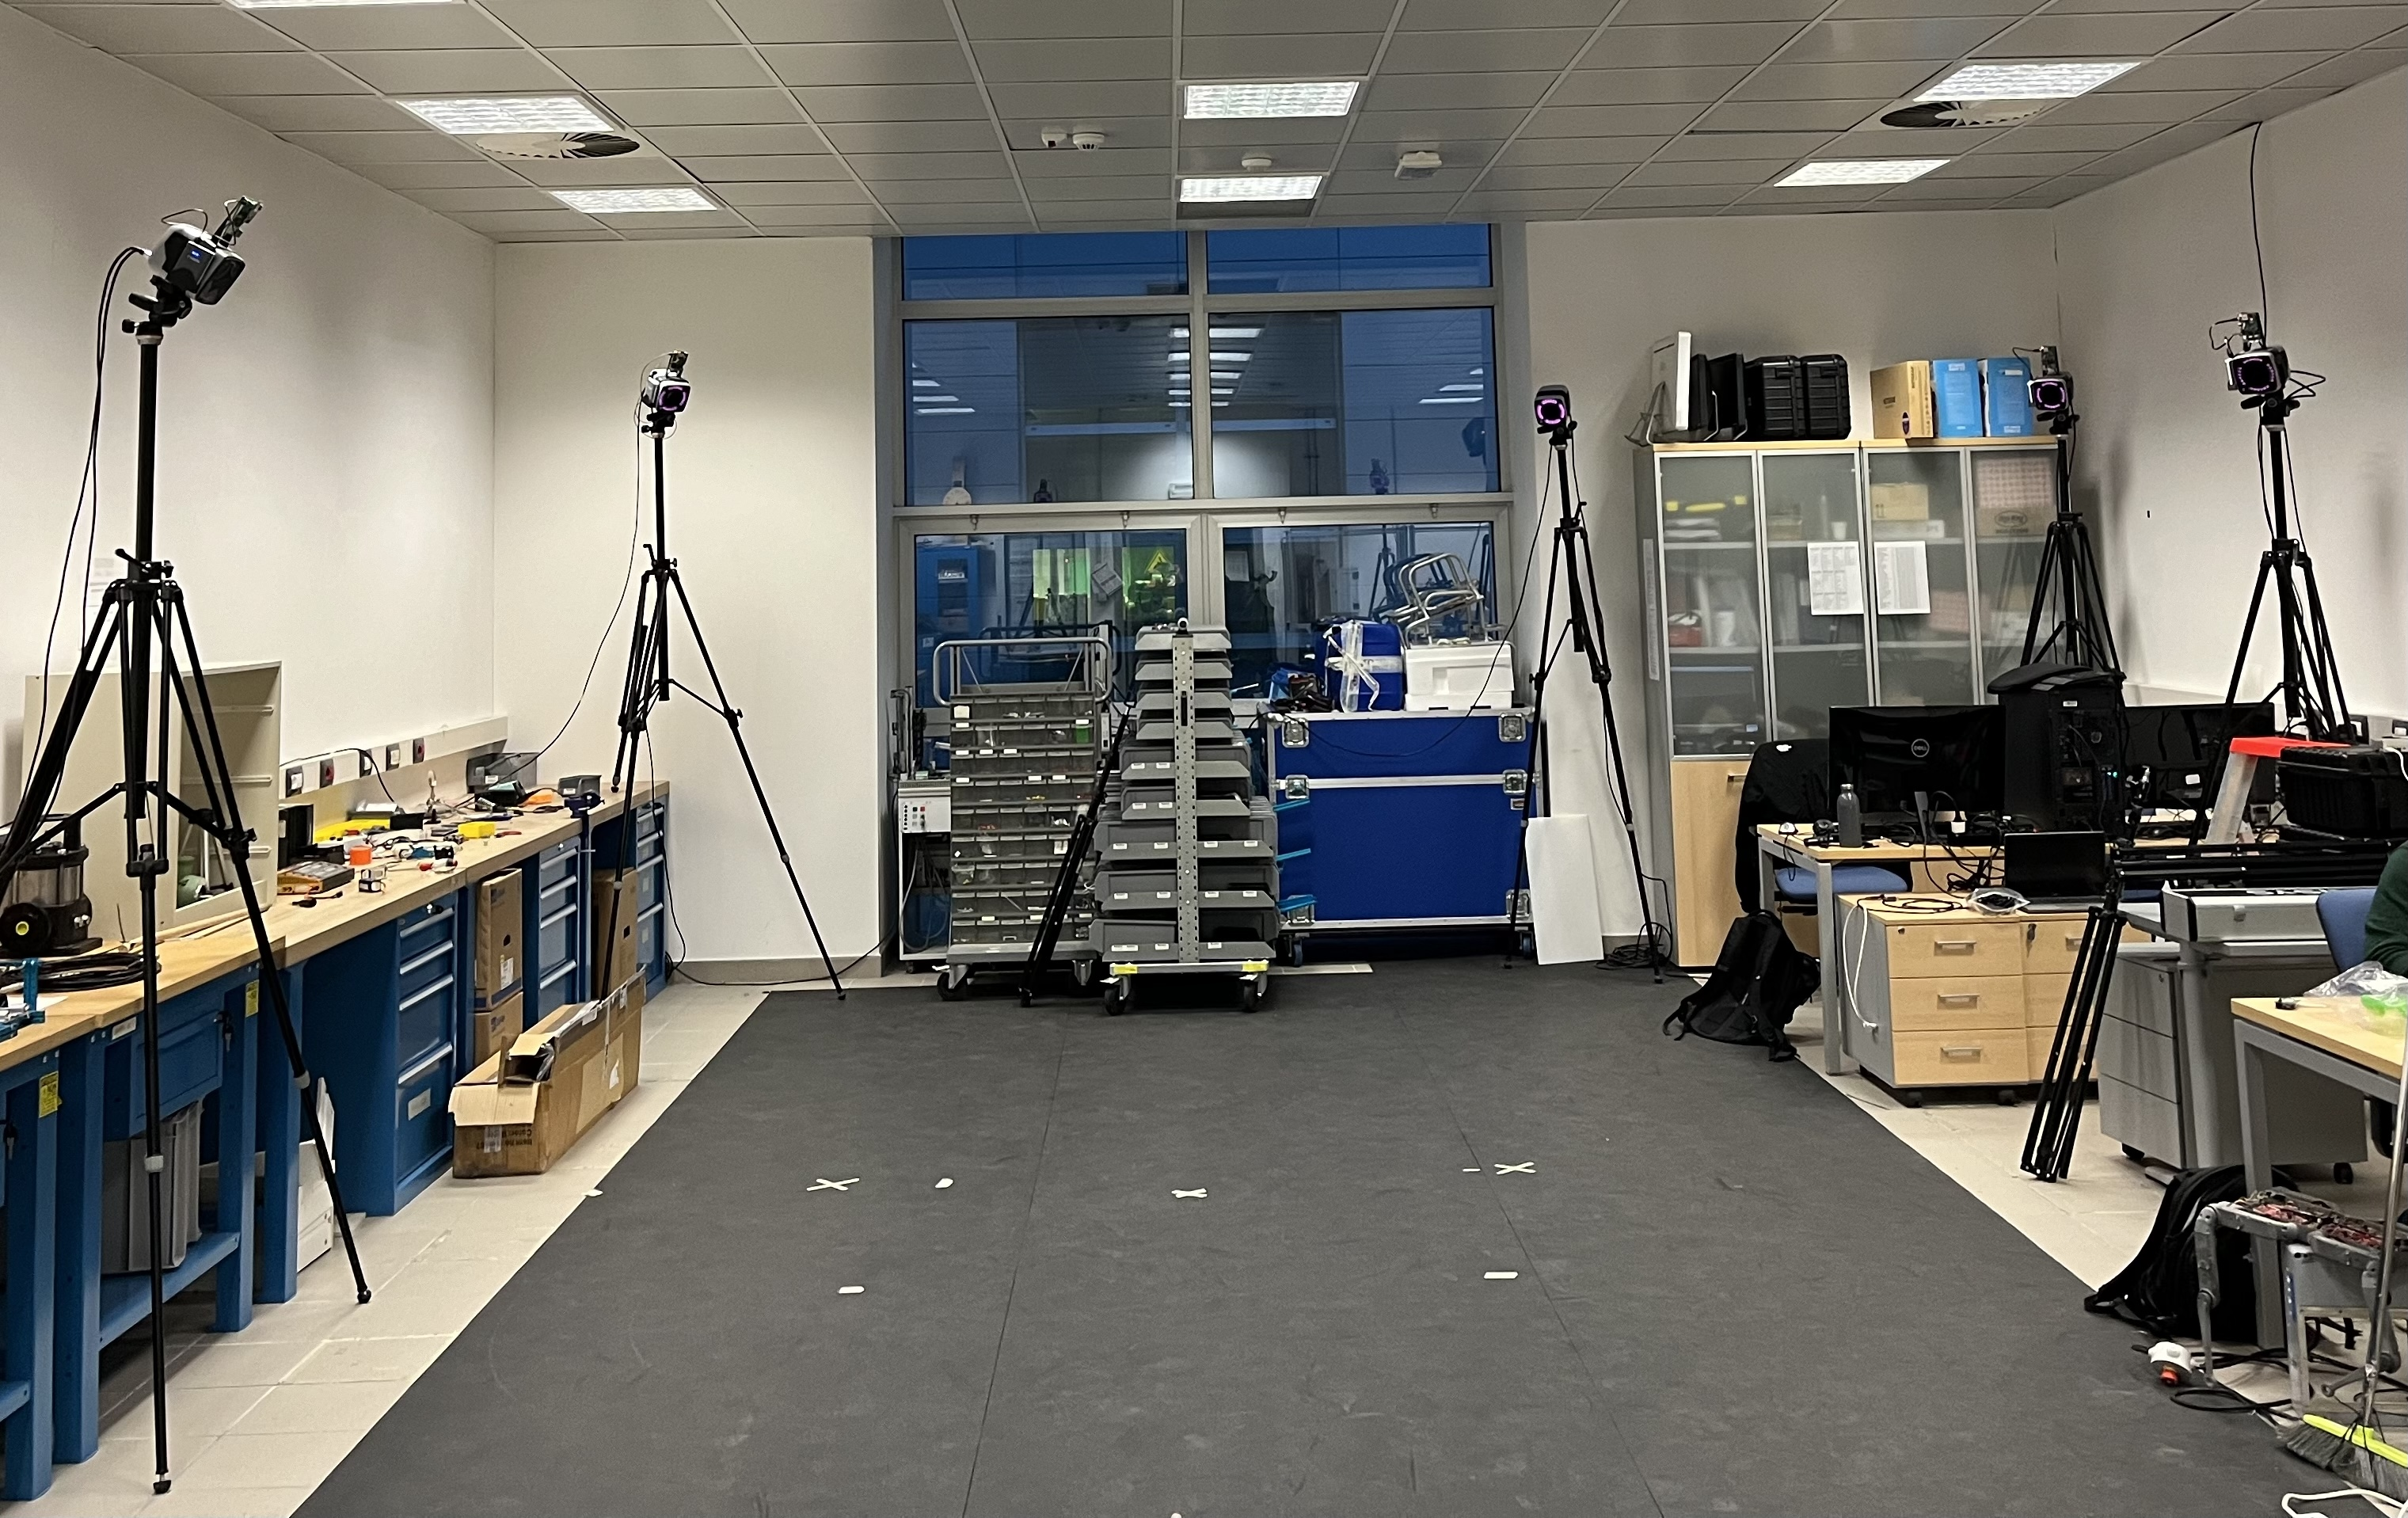
\includegraphics[scale=0.07]{Images/env.JPG}
    \caption{External vision system setup}
    \label{fig:env_hardware}
\end{figure}

\begin{figure}
    \centering
    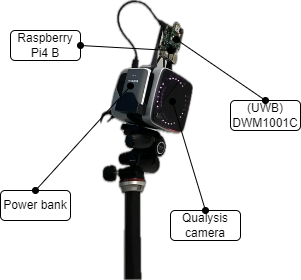
\includegraphics[scale=0.5]{Images/mocap_uwb_hardware_foto.png}
    \caption{Arqus motion capture camera and UWB anchor}
    \label{fig:vision_system}
\end{figure}

\section{External positioning system to PX4 Autopilot}
\label{bridges}

The indoor experimental simulations performed in offboard mode require specific bridges to translate the data given by the external position system into the PX4 message \textbf{VehicleOdometry} \cite{VehicleOdometry} which has to be published in the PX4-ROS2 topic called \textbf{/fmu/in/vehicle\_visual\_odometry}, that it is used to update a PX4-based autopilot's local position estimate (relative to the local origin).

Depending on the reference frame of the external position system, you will need to apply a custom transformation to the pose estimate before sending the \textit{VehicleOdometry} message. In particular, the position estimate has to match the drone reference system, Fig. \ref{fig:ref_frames}, in order to correctly fuse the external position data in the extended Kalman filter (EKF) inside the PX4 autopilot.

If the external position system does not give the full set of data to estimate position and attitude the corresponding field in the message must be set to \textit{Nan} (Not a number) to inform the EKF that the data is not present.

\begin{figure}
    \centering
    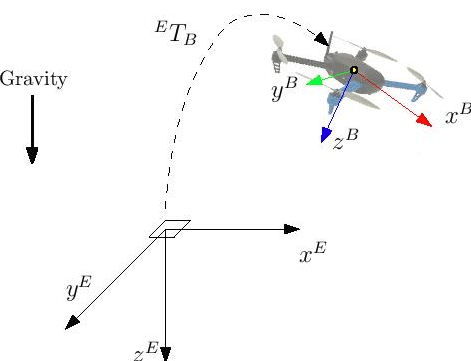
\includegraphics[scale=0.4]{Images/ref_frames.png}
    \caption{Drone reference system}
    \label{fig:ref_frames}
\end{figure}

\subsection{Motion capture (Qualysis)}

To translate the information given by the motion capture system has been used firstly a Qualysis plugin, which connects to the Qualysis server IP address to publish the information into the ROS2 topic \cite{qualisys_ros2}. Then a \textit{ROS2 to PX4 bridge} to translate the message published by the Qualysis plugin in the PX4 message \textit{VehicleOdometry}.

\subsection{Ultra WideBand and Sonar}

To perform the Ultra WideBand and Sonar simulation two different bridges are needed, one for the UWB module and the other for the ultrasonic sensor.

The UWB bridge aims to connect the USB port at which the UWB module is connected, read the data collected by the sensor, perform the differential time difference of arrival (DTDOA) algorithm to convert the data read in local coordinates, and fill the PX4 message \textit{VehicleOdometry}.

The MB1202 bridge instead aims to connect to the I2C address bus where the ultrasonic sensor is connected, reads the data, and fills the PX4 message \textit{VehicleOdometry}.

\section{Simulation} 
\label{simulations}
\subsection{Simulation environment}

The simulation environment used to simulate the physical interaction between the drone and the real world is \textbf{Gazebo classic}, shown in Fig. \ref{fig:Gazebo-classic}, which is an open-source 3D robotics simulator. Gazebo Classic integrated the ODE physics engine, OpenGL rendering, and support code for sensor simulation and actuator control.

In particular, it has been used the Gazebo Software In The Loop (SITL) feature present in the PX4-Autopilot package. This feature allows the interaction with a simulated vehicle and flight stack with the same characteristics as the real system.

\begin{figure}
    \centering
    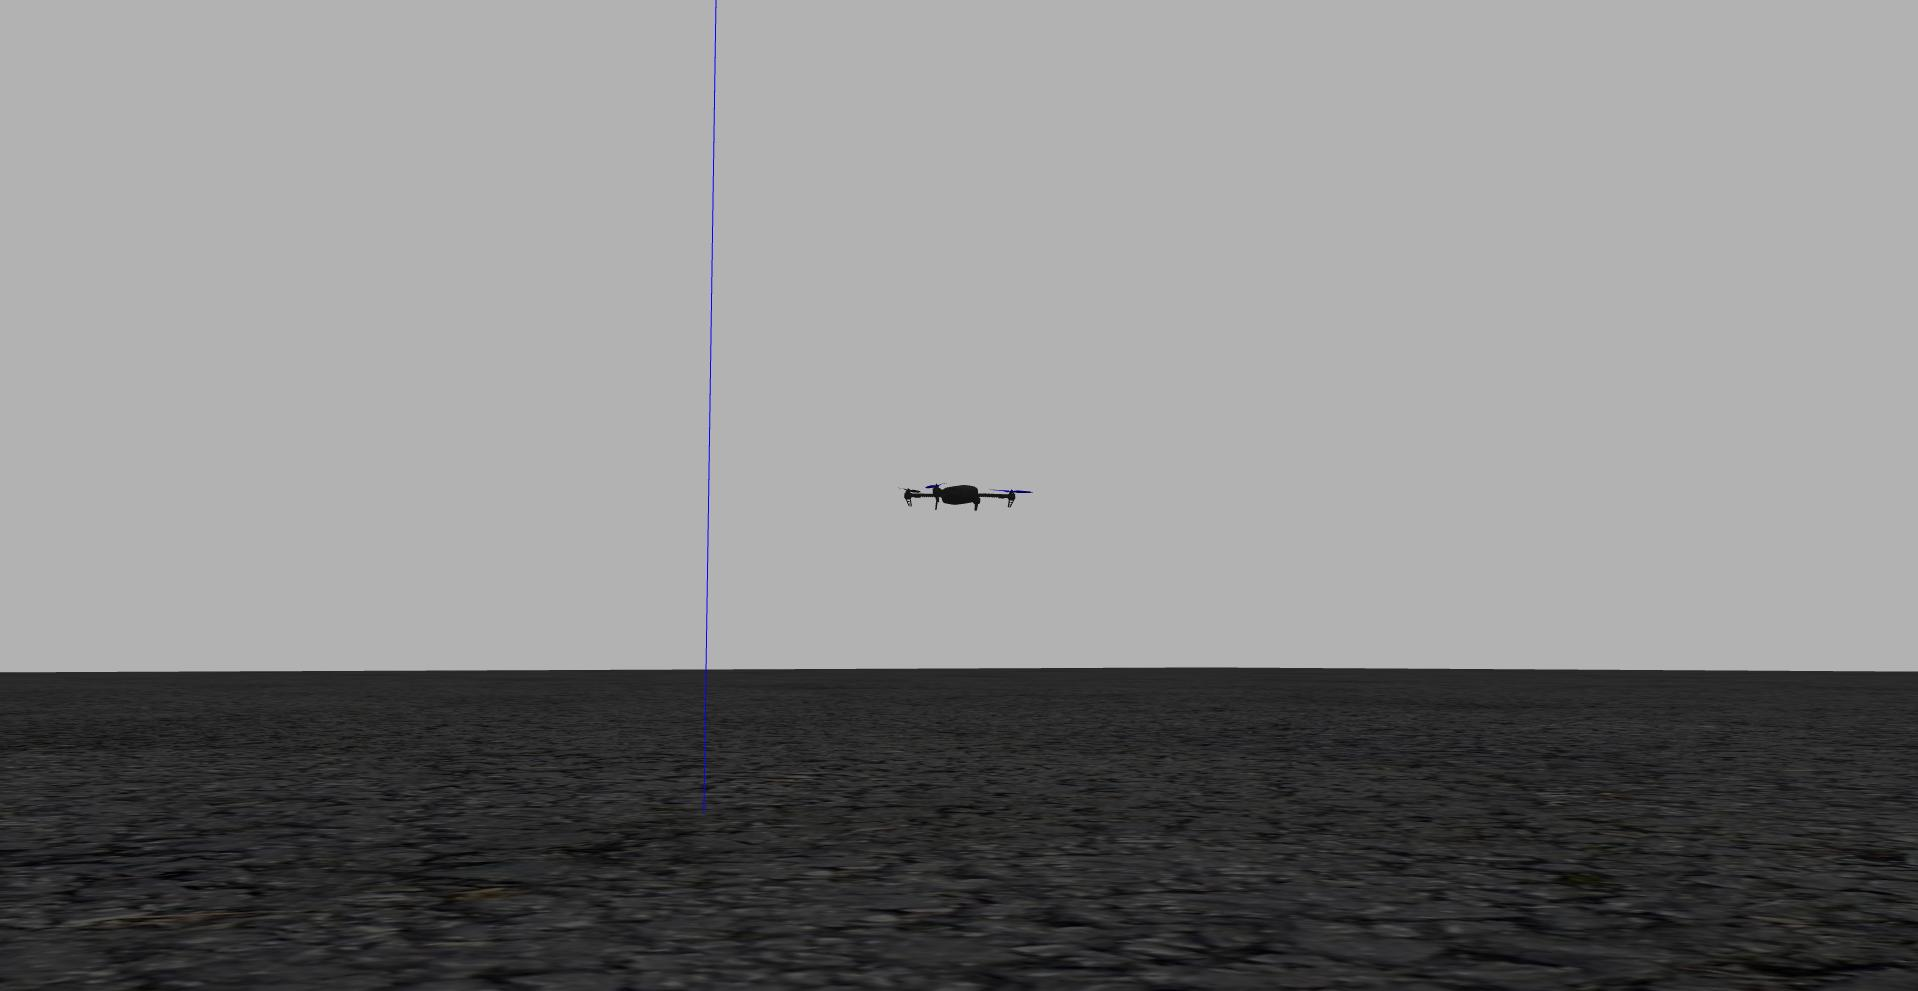
\includegraphics[scale=0.13]{Images/gzclient_camera.jpg}
    \caption{Gazebo-classic simulation environment}
    \label{fig:Gazebo-classic}
\end{figure}

\subsection{Plugins} \label{sec:plugin}

The PX4-Autopilot package contains several plugins to control the vehicle and to simulate a GPS noisy signal. 

To simulate the GPS positioning system has been used the default plugin, while to simulate the external position systems used for the indoor simulations two different plugins have been implemented, one to simulate the Motion capture system and one to simulate the ultra-wide band system.

The Motion capture plugin \cite{mocap_plugin} aims to retrieve the drone position and attitude with respect to the Gazebo origin reference frame, translate the information in a \textbf{PoseStamped} geometry message, the message type published by the Qualysis server, and publish it in a ROS2 topic.

The Ultra WideBand plugin \cite{uwb_plugin}, related to the scientific work \cite{uwb_plugin_paper} and modified accordingly to this work, instead aims to simulate a UWB infrastructure. In particular, can define the position of the anchors in the simulated word and the position of the tag, once the simulation is started two ROS2 topics are published giving one the position and orientation of the anchors and the other one the anchor ID and its distance from the tag.

\subsection{Program structure}

The code used to control the vehicle has the same structure for all three different positioning techniques and it is shown in Algorithm \ref{alg:callback}. The same program has been implemented using two different programming languages, \textbf{C++} and \textbf{Python}.

Firstly it initialise a list of points describing the trajectory that the drone has to follow (a point is completely described with the x, y and z coordinates) and initialise to zero the \textit{offboard\_setpoint\_counter\_} counter which is incremented every cycle.

The timer callback cycle starts by sending the $arm()$ and $takeoff()$ commands when the \textit{offboard\_setpoint\_counter\_} is equal to 0, so only the first cycle iteration, lines 1 to 4.

Then when the vehicle has completed the takeoff command and the point list is not empty the timer callback calls \textit{publish\_offboard\_control\_mode()} and \textit{publish\_trajectory\_setpoint()} to send \textit{OffboardControlMode} and \textit{TrajectorySetpoint} messages to PX4, lines 5 to 9, which inform the PX4 to set the offboard mode and publish the reference trajectory to follow.

At the end when the point list is empty, which means the vehicle has completed the reference trajectory, the \textit{land()} command is sent, and when the landing command is finished the disarm command concludes the callback. 

\RestyleAlgo{ruled}
\begin{algorithm}[hbt!]

\caption{timer\_callback()}\label{alg:callback}
\tcp{Arm and takeoff}
\If{$offboard\_setpoint\_counter\_ == 0$}
{
    $arm()$ \\
    $takeoff()$ 
}
\tcp{Trajectory setpoint}
\If{$takeoff\_finished == 1 \ and \ len(point\_list) != 0$}
{
    $publish\_vehicle\_command(VehicleCommand.$ 
    $VEHICLE\_CMD\_DO\_SET\_MODE, 1., 6.)$ \\
    $publish\_offboard\_control\_mode()$ \\
    $publish\_trajectory\_setpoint()$
}
\tcp{Land (when the list is empty and all points are reached)}
\If{$len(point\_list) == 0$}
{
    $land()$
}
\tcp{Disarm}
\If{$landing\_flag == true$}
{
    $disarm()$
}
$offboard\_setpoint\_counter\_ += 1$
\end{algorithm}

The \textit{publish\_trajectory\_setpoint()} function is described in Algorithm \ref{alg:trj_setpoint}. The algorithm checks firstly if the point list is not empty, then it fills the \textbf{TrajectorySetpoint} message with the point and the velocity Setpoint, and publishes the message in the corresponding topic. When the distance between the reference point and the drone position is less than the tolerance radius the point is considered reached and it is deleted from the point list.

\RestyleAlgo{ruled}
\begin{algorithm}[hbt!]
\caption{publish\_trajectory\_setpoint()}\label{alg:trj_setpoint}
$msg = TrajectorySetpoint()$ \\
$point = self.point\_list$ \\
$range = self.range$  \\
\tcp{check the list is not empty}
\If{$len(point) > 0$}{   
    $msg.position = [point[0].x, point[0].y, point[0].z]$ \\
    $msg.velocity = [self.velx, self.vely, self.velz]$ \\
    \tcp{point is reached}
    \If{$self.distance(point[0]) <= range$}{   
        \tcp{delete the reached point from the list}
        $point.pop(0)$  
    }
}
$msg.timestamp = int(Clock().now().nanoseconds / 1000)$ \\
$self.trajectory\_setpoint\_publisher\_.publish(msg) $
\end{algorithm}

\subsection{Software in the loop Simulations}

\subsubsection{GPS simulation}

The GPS simulation is the simplest one since is the \textit{default simulation} that can be done with the PX4-Autopilot package. In particular, the drone estimates its position and attitude using a noisy GPS signal coupled with the Pixhawk onboard sensors, which are accelerometer, gyroscope, barometer, and magnetometer. 

In Fig. \ref{fig:SITL_GPS_TIME} the XYZ coordinates of the drone, mapped as North-East-Down in the inertial navigation frame, are shown. In particular, the \textit{Setpoint} to follow (reference trajectory), the \textit{Estimated} position by the PX4 and the \textit{Ground Truth} position broadcasted by the simulator.

\begin{figure}
    \centering
    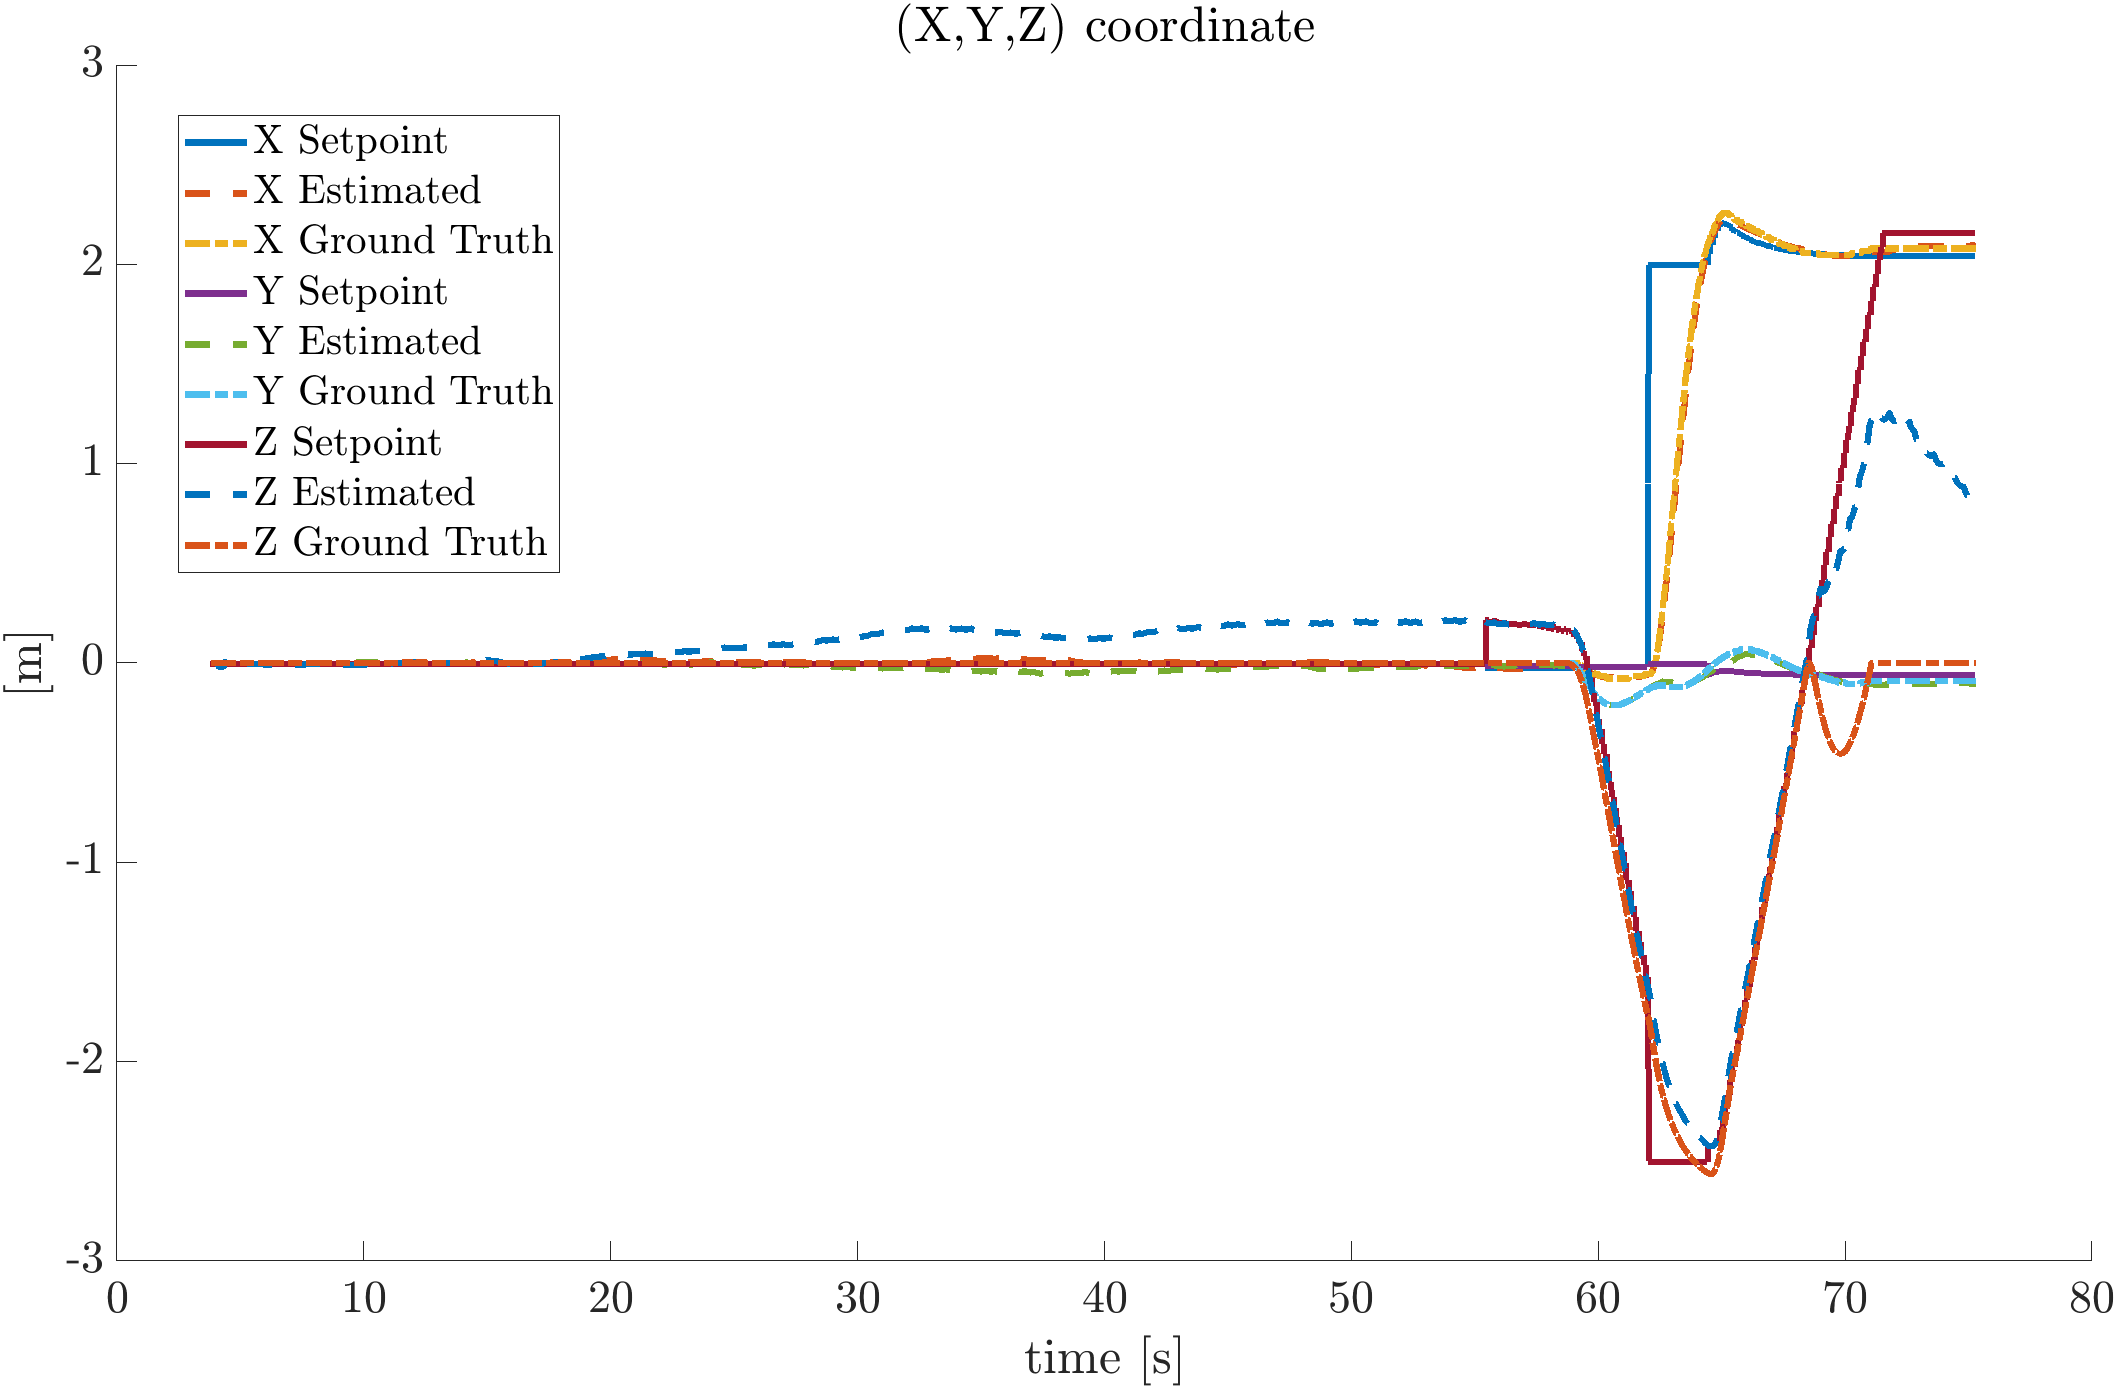
\includegraphics[scale=0.2]{Images/SITL_GPS/XYZ_Sitl_gps_time.png}
    \caption{(X,Y,Z) Coordinate in time, in GPS SITL simulation}
    \label{fig:SITL_GPS_TIME}
\end{figure}

As we can see from Fig. \ref{fig:SITL_GPS}, the drone follows quite well the reference trajectory, however does not recognise well the landing, since the internal estimator of PX4 believes that it is underground: this is not a problem because it happens only after the vehicle has already landed.

\begin{figure}
    \centering
    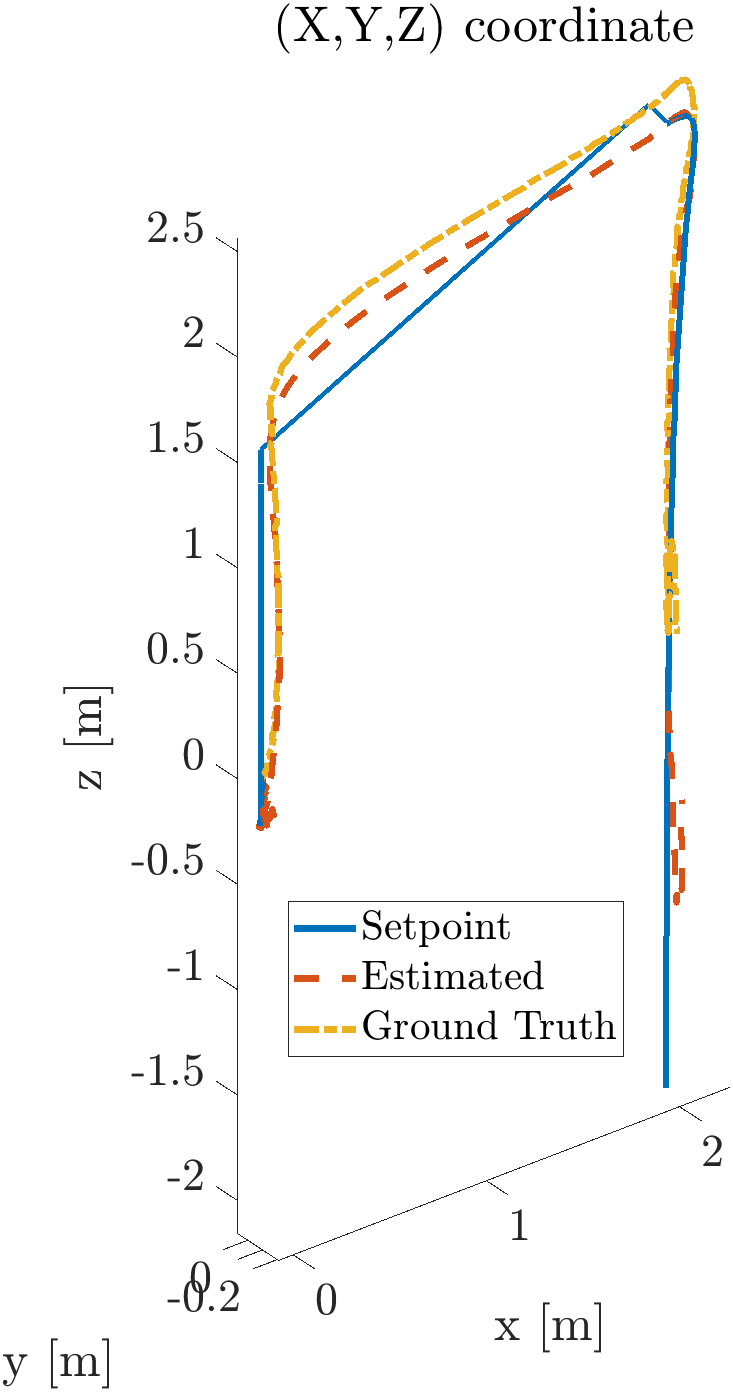
\includegraphics[scale=0.2]{Images/SITL_GPS/XYZ_Sitl_gps.png}
    \caption{(X,Y,Z) Coordinate in GPS SITL simulation}
    \label{fig:SITL_GPS}
\end{figure}

\subsubsection{Motion capture simulation}

To perform the MoCap simulations the \textit{Motion capture plugin} described in section \ref{sec:plugin} was used, obtaining the local coordinates of the drone through the ROS2 topic \textit{/Drone/pose}. 

To simulate the Motion capture test the sensors used in the GPS simulation have been disabled from the estimation. In particular, the GPS information and the barometer information.

The information given by the Motion capture plugin is fused in the PX4-Autopilot by publishing a \textit{VehicleOdometry} message in the ROS2 topic \textit{/fmu/in/vehicle\_visual\_odometry} as described in the section \ref{bridges}.

In Fig. \ref{fig:SITL_MOCAP_TIME} the XYZ coordinates of the drone, mapped as North-East-Down in the inertial navigation frame, are shown. As for the GPS simulation, the \textit{Setpoint}, the \textit{Estimated} and the \textit{Ground Truth} positions broadcasted by the simulator are shown.

\begin{figure}
    \centering
    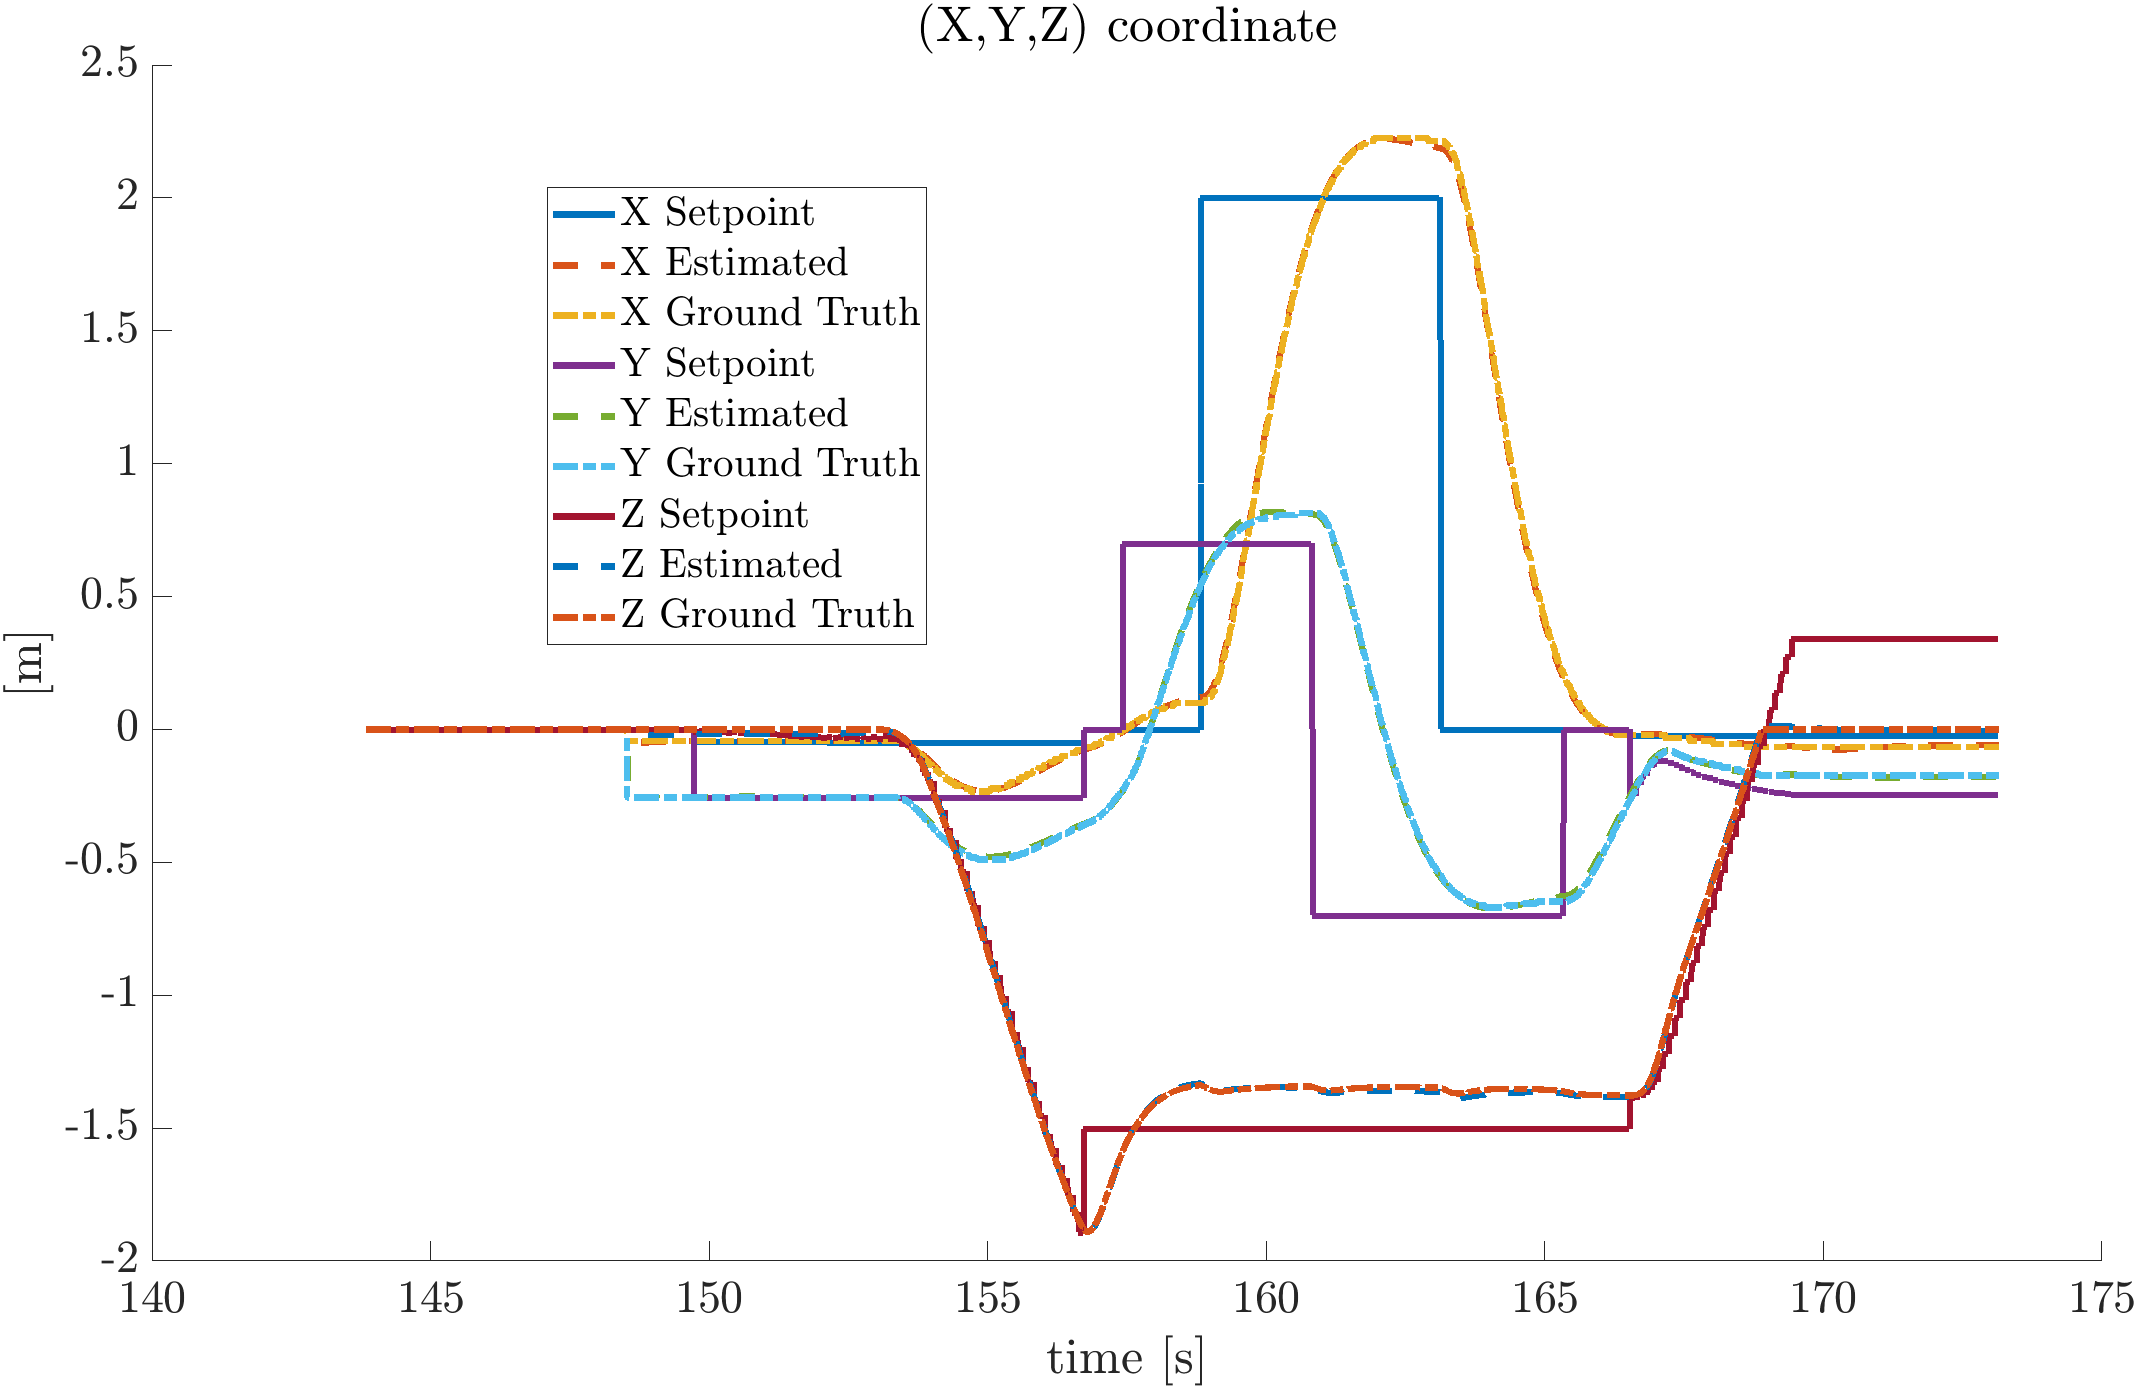
\includegraphics[scale=0.23]{Images/SITL_MOCAP/xyz_sitl_mocap_time.png}
    \caption{(X,Y,Z) Coordinate in time, in MoCap SITL simulation}
    \label{fig:SITL_MOCAP_TIME}
\end{figure}

In Fig. \ref{fig:SITL_MOCAP} the 3D trajectory followed by the drone is represented. As can be seen, the drone follows very well the Setpoint trajectory.

\begin{figure}
    \centering
    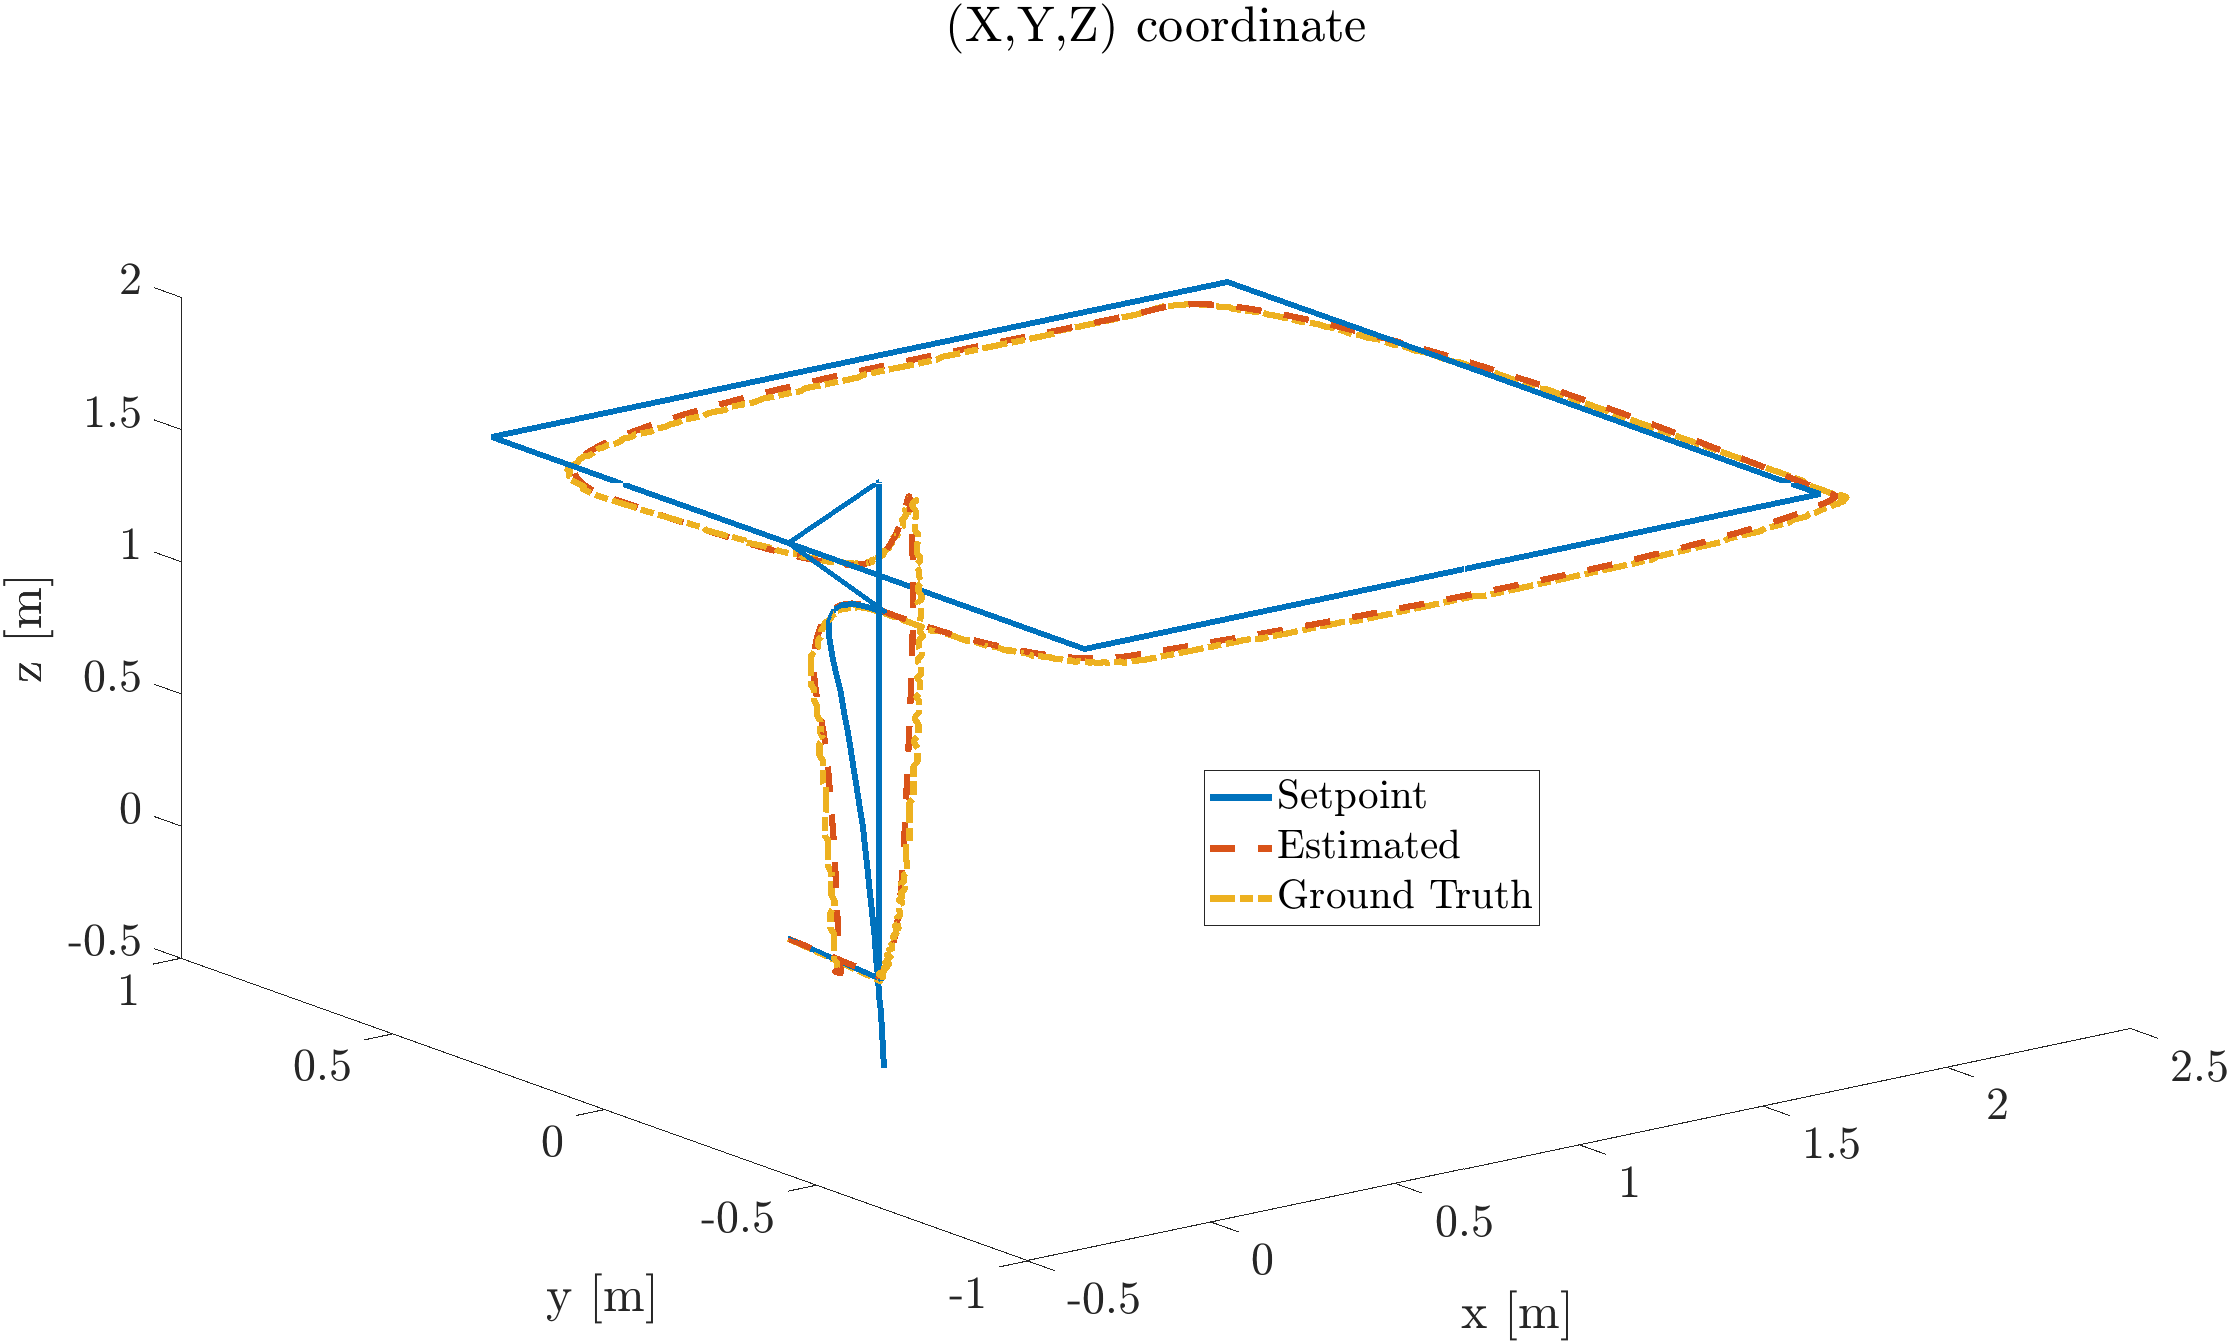
\includegraphics[scale=0.20]{Images/SITL_MOCAP/xyz_sitl_mocap.png}
    \caption{(X,Y,Z) Coordinate, in MoCap SITL simulation}
    \label{fig:SITL_MOCAP}
\end{figure}

\subsubsection{Ultra WideBand simulation}

This simulation aims to test the multilateration algorithm presented above, after implementing it in Python. 

To do this the UWB plugin shown in section \ref{sec:plugin} was used, obtaining the coordinates of each anchor and the distance between the latter and the tag. Then, given these values, it is possible to solve iteratively equation \ref{eq:mult}, achieving the drone position at any time. The solution in equation \ref{eq:lstsqr} is directly reached by the least squares minimisation using the Python function \textit{numpy.linalg.lstsq}.

As for the MoCap simulation, the GPS and the barometer information have been disabled to simulate an indoor application, and also in this case the position obtained through the multilateration algorithm is fused in the PX4-Autopilot by publishing a \textit{VehicleOdometry} message in the ROS2 topic \textit{/fmu/in/vehicle\_visual\_odometry}. 

To assess the algorithm accuracy, the computed UWB position is compared with the Ground truth, provided by the simulation environment. As it is possible to infer in Fig. \ref{fig:uwb_sim}, the two signals are on the whole superimposed: considering that the plugin used includes noise to simulate a real signal and that the solution is not exact but the result of a minimisation, it can be concluded that the multilateration algorithm used provides a reliable position. 

\begin{figure}
    \centering
    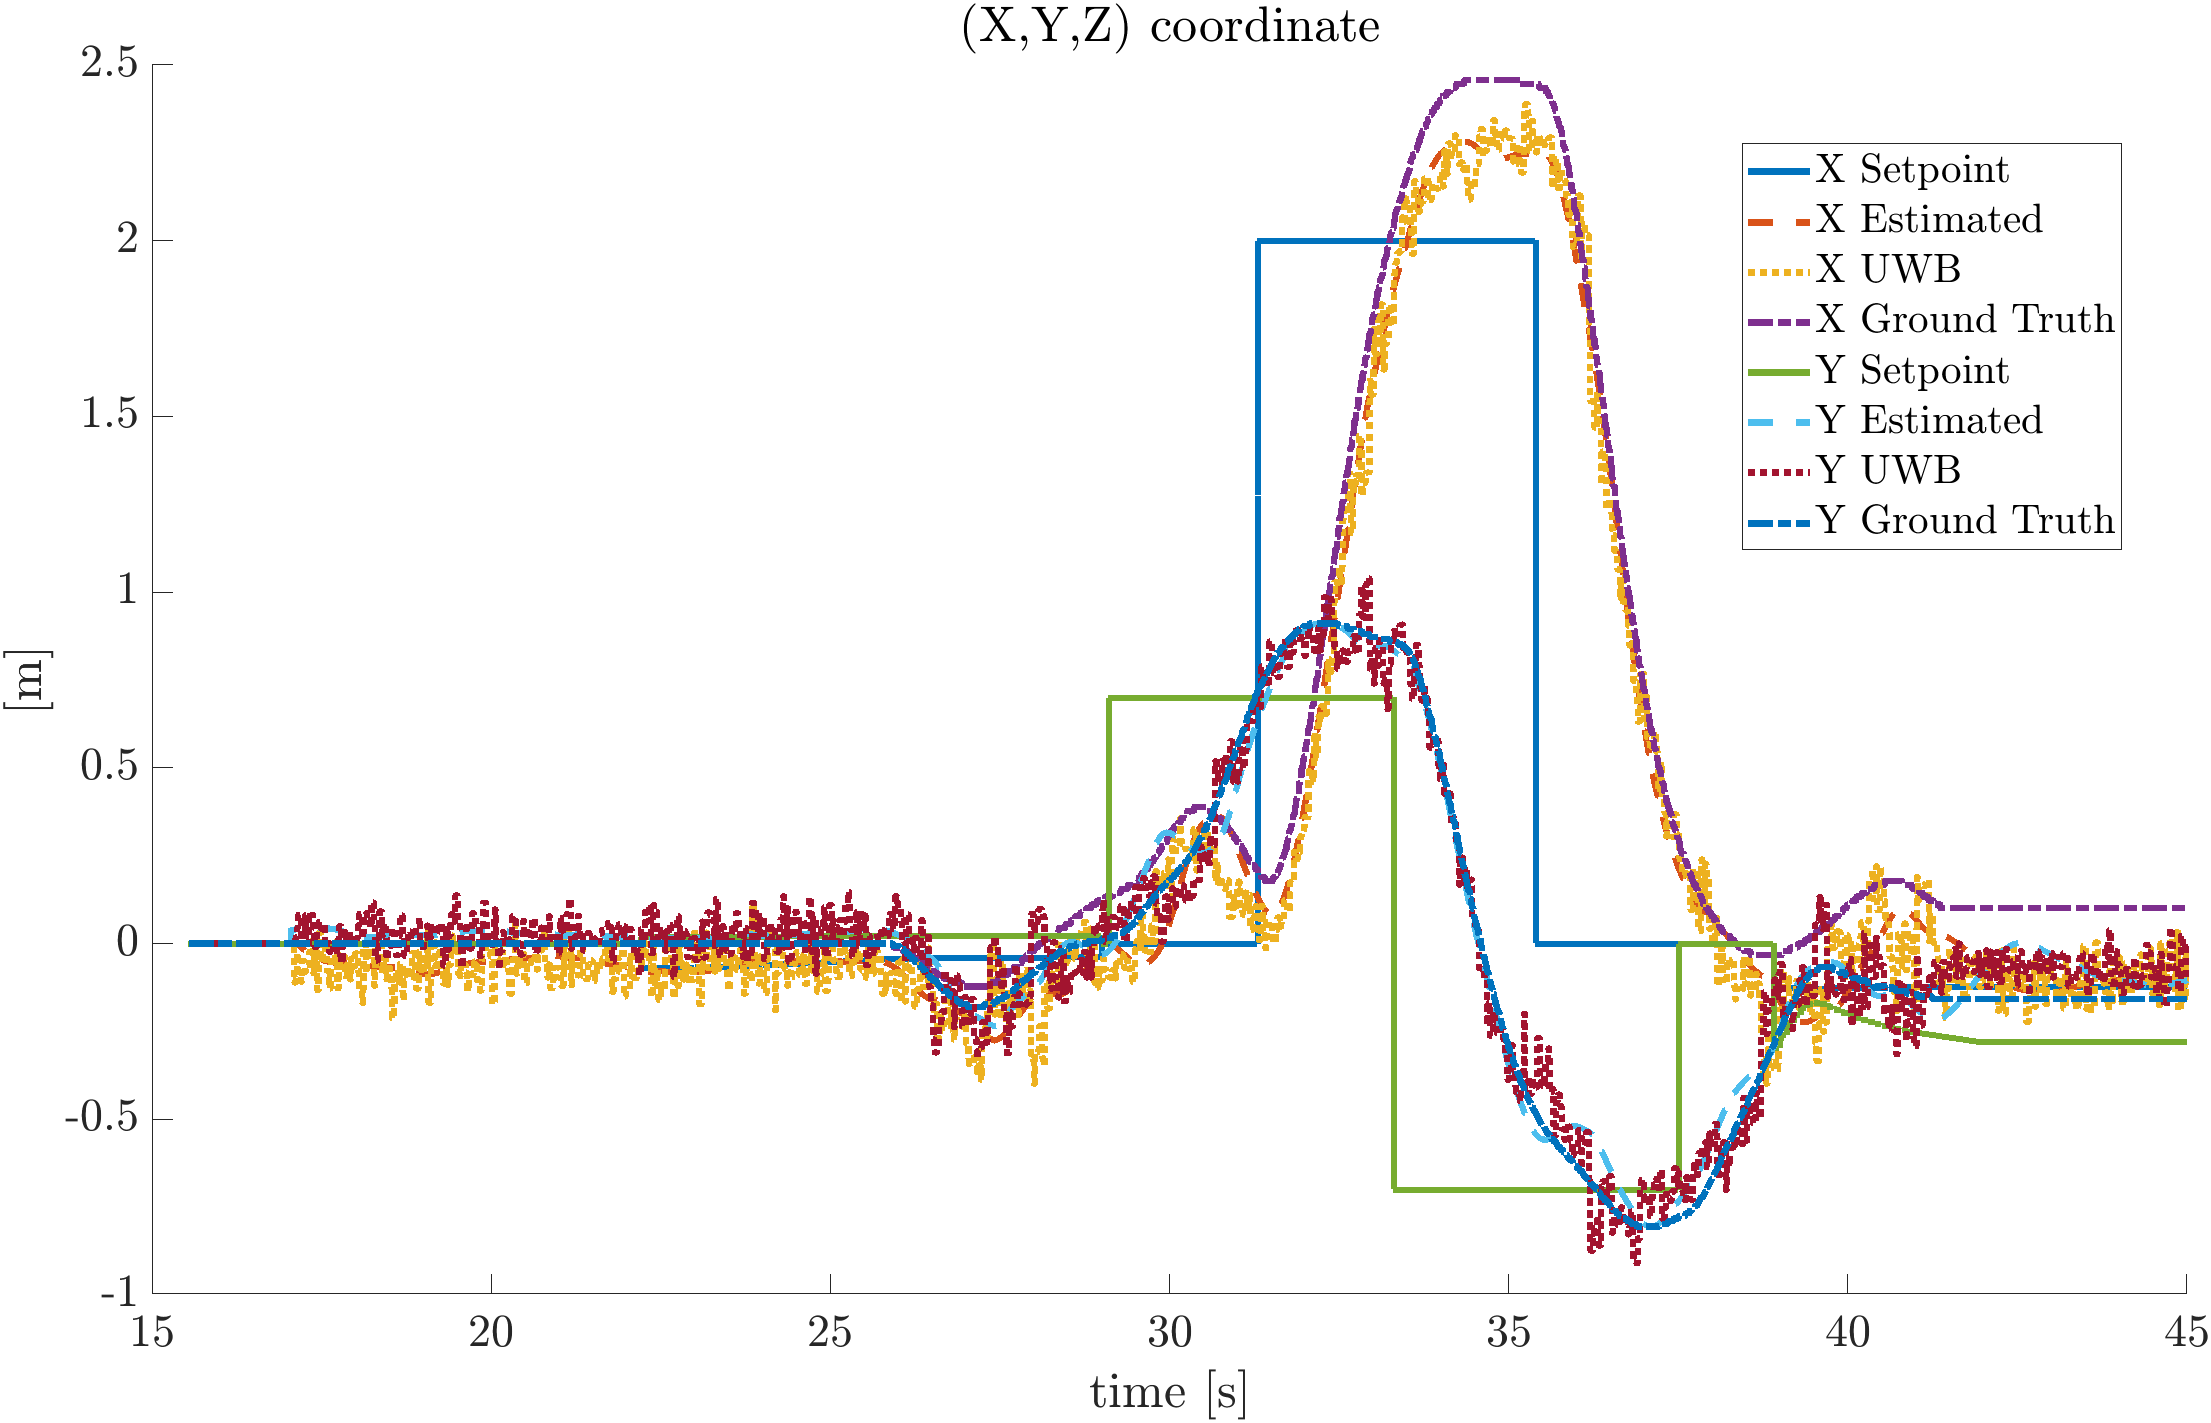
\includegraphics[scale=0.2]{Images/SITL_UWB/xy_sitl_uwb_un_time.png}
    \caption{Comparison of x and y position of the drone over time, one obtained using a multilateration algorithm and the second provided by the simulation environment.}
    \label{fig:uwb_sim}
\end{figure}


\subsection{Hardware in the loop simulation}

Hardware-in-the-Loop (HITL or HIL) is a simulation mode in which normal PX4 firmware is run on real flight controller hardware. This approach has the benefit of testing most of the actual flight code on the real hardware \cite{hitl}, and can validate the interaction between the hardware and software components of the drone, identifying any compatibility issues or communication problems among them. The flight controller of the vehicle is connected to Gazebo, which is running on a development computer, via USB. Then, HITL configuration is selected using \textit{QGroundControl}: in this way all real sensors and motors will not activate, using instead the imitated ones by the simulation environment. The program is launched on the companion board (Raspberry Pi 4B) that communicates with the Pixhawk to perform the flight, using its real firmware previously flashed. 

The achieved results confirm that the hardware architectures and their relative communication work properly. The plots concerning these tests have been omitted since they are quite similar to the ones obtained in SITL simulations.

\section{Experimental results}
\label{experimental}

In all the experimental tests presented below the safety conditions have been met, keeping the drone tied to a stick and ensuring to be prepared with the radio controller, in order to take control of the vehicle if necessary. \\

\subsection{GPS test results}

The experimental test using GPS as a positioning method was accomplished outdoor, choosing a place away from buildings to avoid drifting of the signal and to satisfy the requirements indicated in section \ref{Environment-setup}. 

Fig. \ref{fig:gps_results} shows a first attempt trajectory completed by the drone. As it is possible to infer by the several turns around the set points, it was difficult to reach them exactly: this is due to a too strict tolerance between the vehicle's position and the point to be achieved. In a second attempt, widening the tolerance, it was easier to reach the required points. This aspect must be taken into account when working with GPS, which presents a not negligible error, which makes it difficult to command the drone in position.

Another thing that it is possible to notice in Fig. \ref{fig:gps_results} is that the initial position of the drone is not at the origin, which is reached later. As it is reported in PX4 User Guide \cite{VehicleLocalPos}, the coordinate system origin is the vehicle position at the time when it was started: the shift means that the drone was slightly moved after being turned on.

\begin{figure}
    \centering
    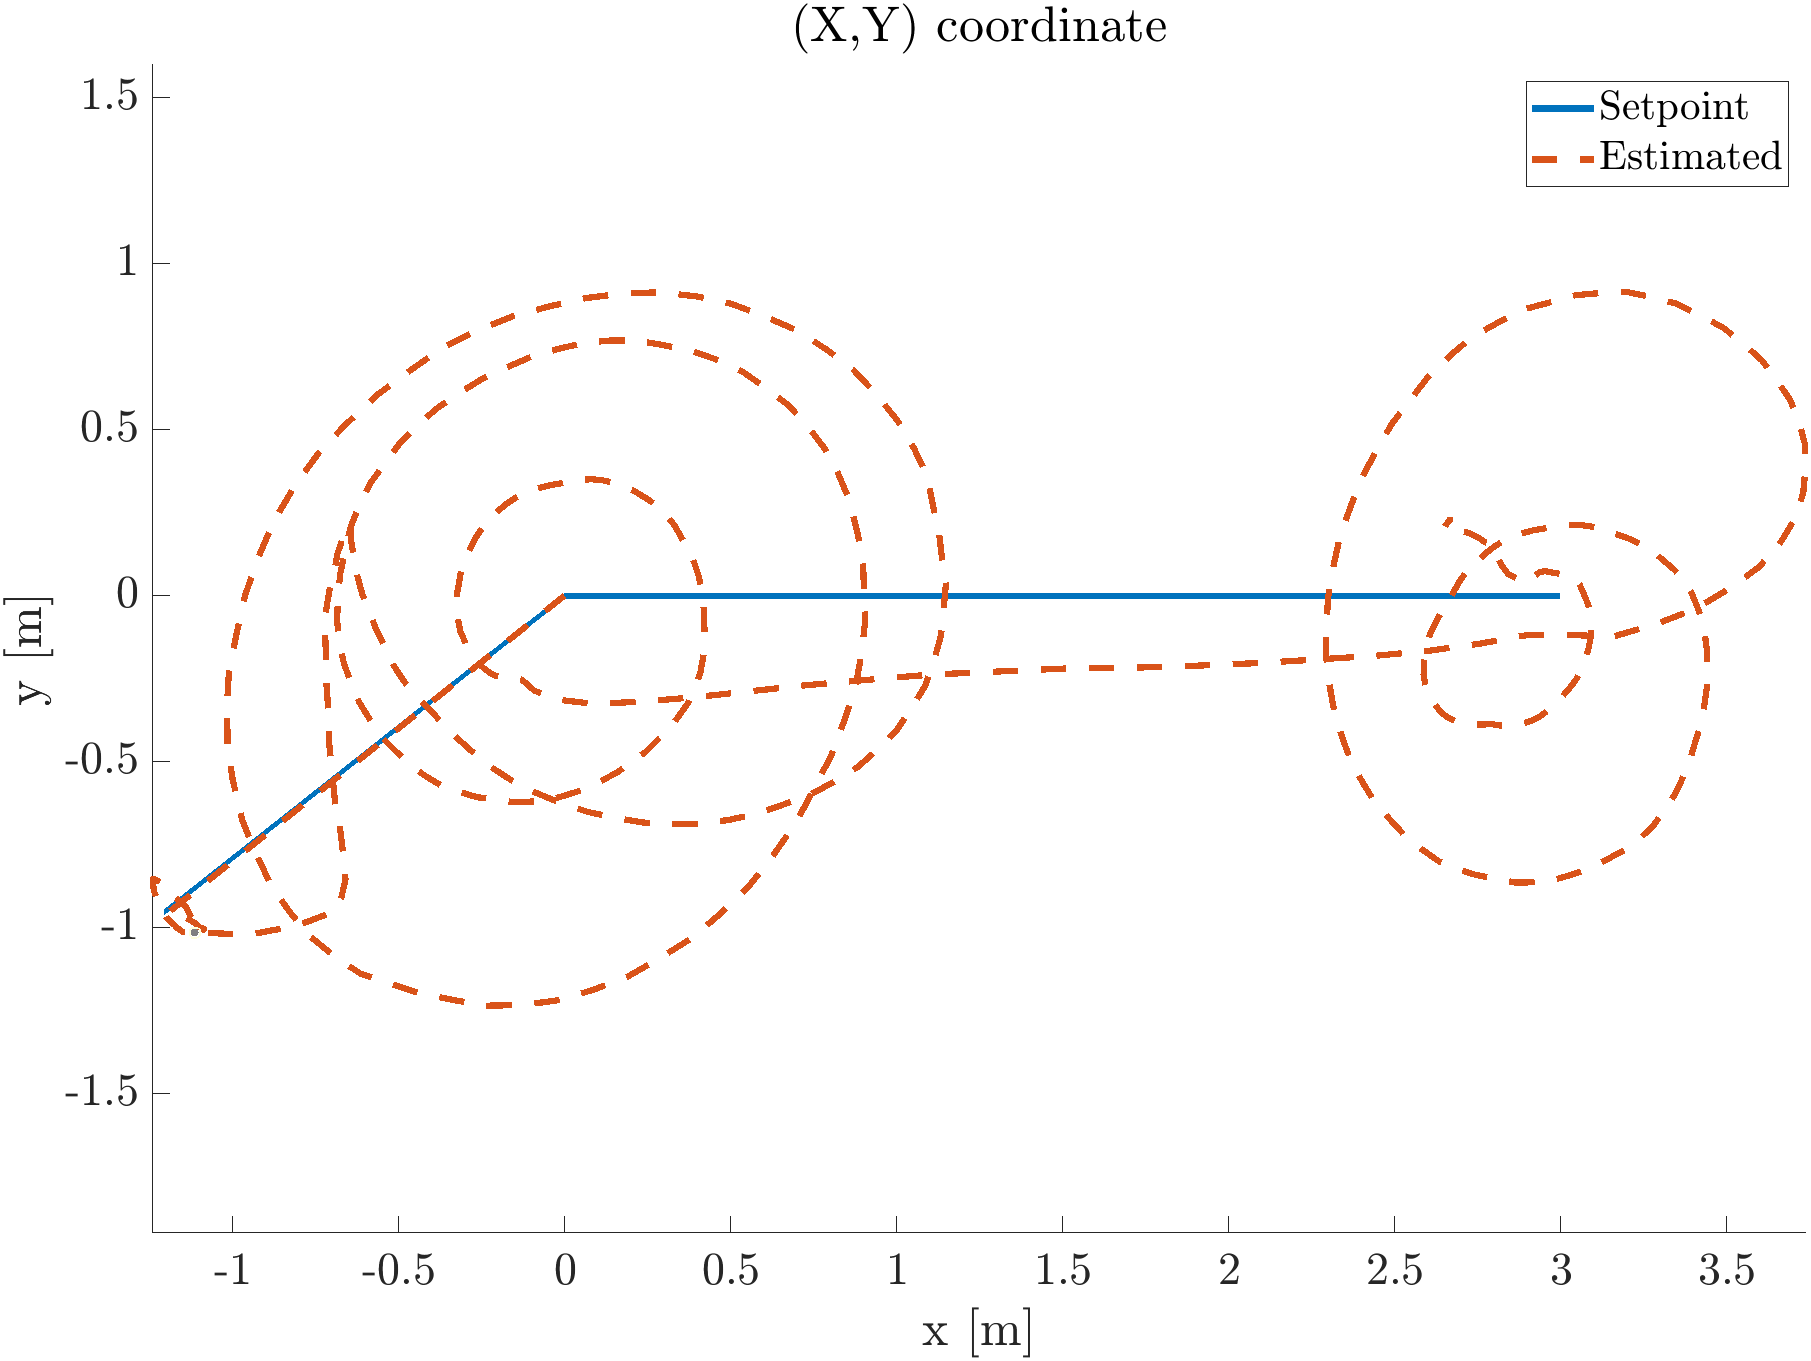
\includegraphics[scale=0.2]{Images/xy_gps.png}
    \caption{GPS experimental results.}
    \label{fig:gps_results}
\end{figure}

\subsection{Motion capture test results}

The experimental test concerning the motion capture simulations has been carried out using Qualysis cameras, as introduced in the section \ref{Environment-setup}. The drone has been equipped with five markers and the body \textbf{Drone} has been created in the Qualysis server, as can be seen in Fig. \ref{fig:mocap_interface}.

\begin{figure}
    \centering
    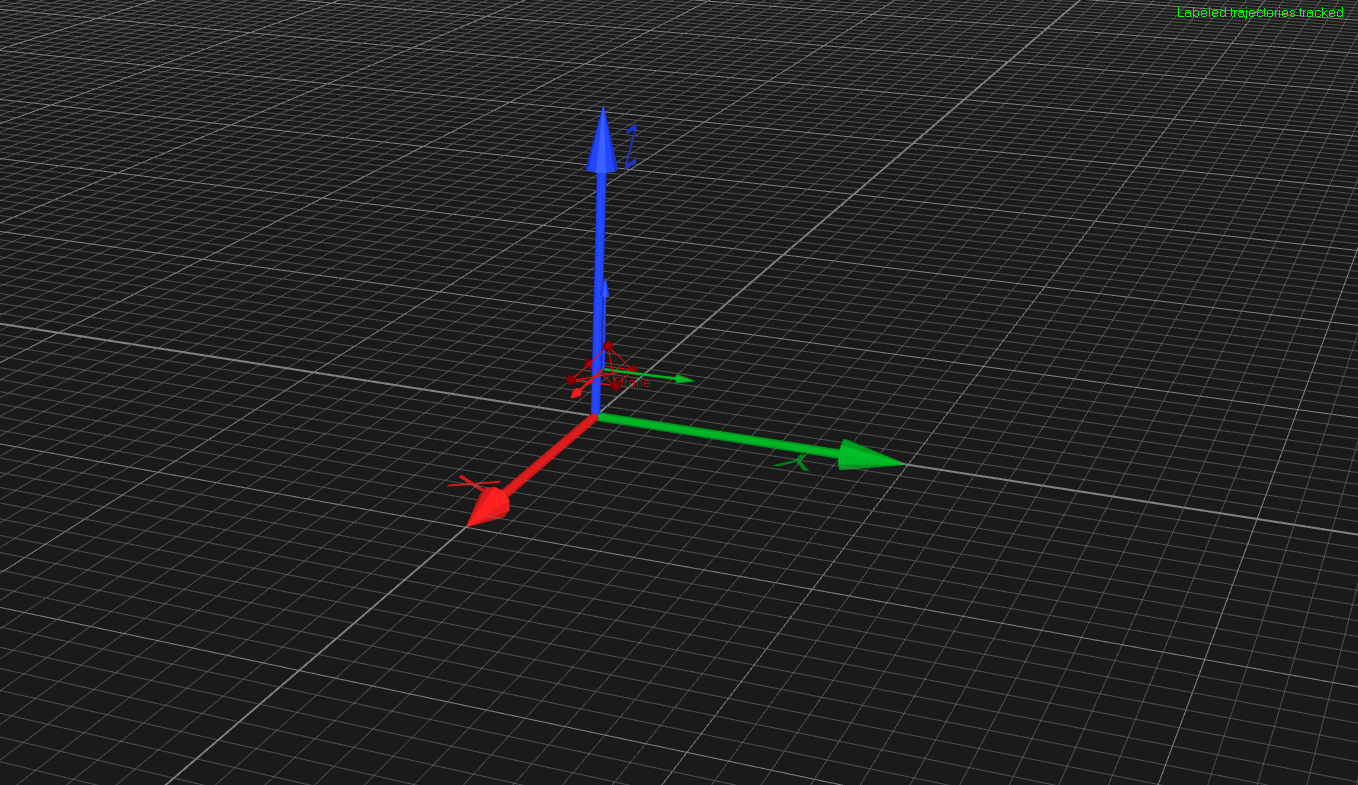
\includegraphics[scale=0.15]{Images/mocap_interface.png}
    \caption{Motion capture interface}
    \label{fig:mocap_interface}
\end{figure}

In Fig. \ref{fig:mocap_test} is represented the 3D trajectory followed by the drone. In particular, the \textit{Setpoint} trajectory that the drone has to follow (a squared trajectory), the position estimated from PX4, using the MoCap signal coupled with the IMU data, and the Motion capture trajectory captured by the Qualysis system.

\begin{figure}
    \centering
    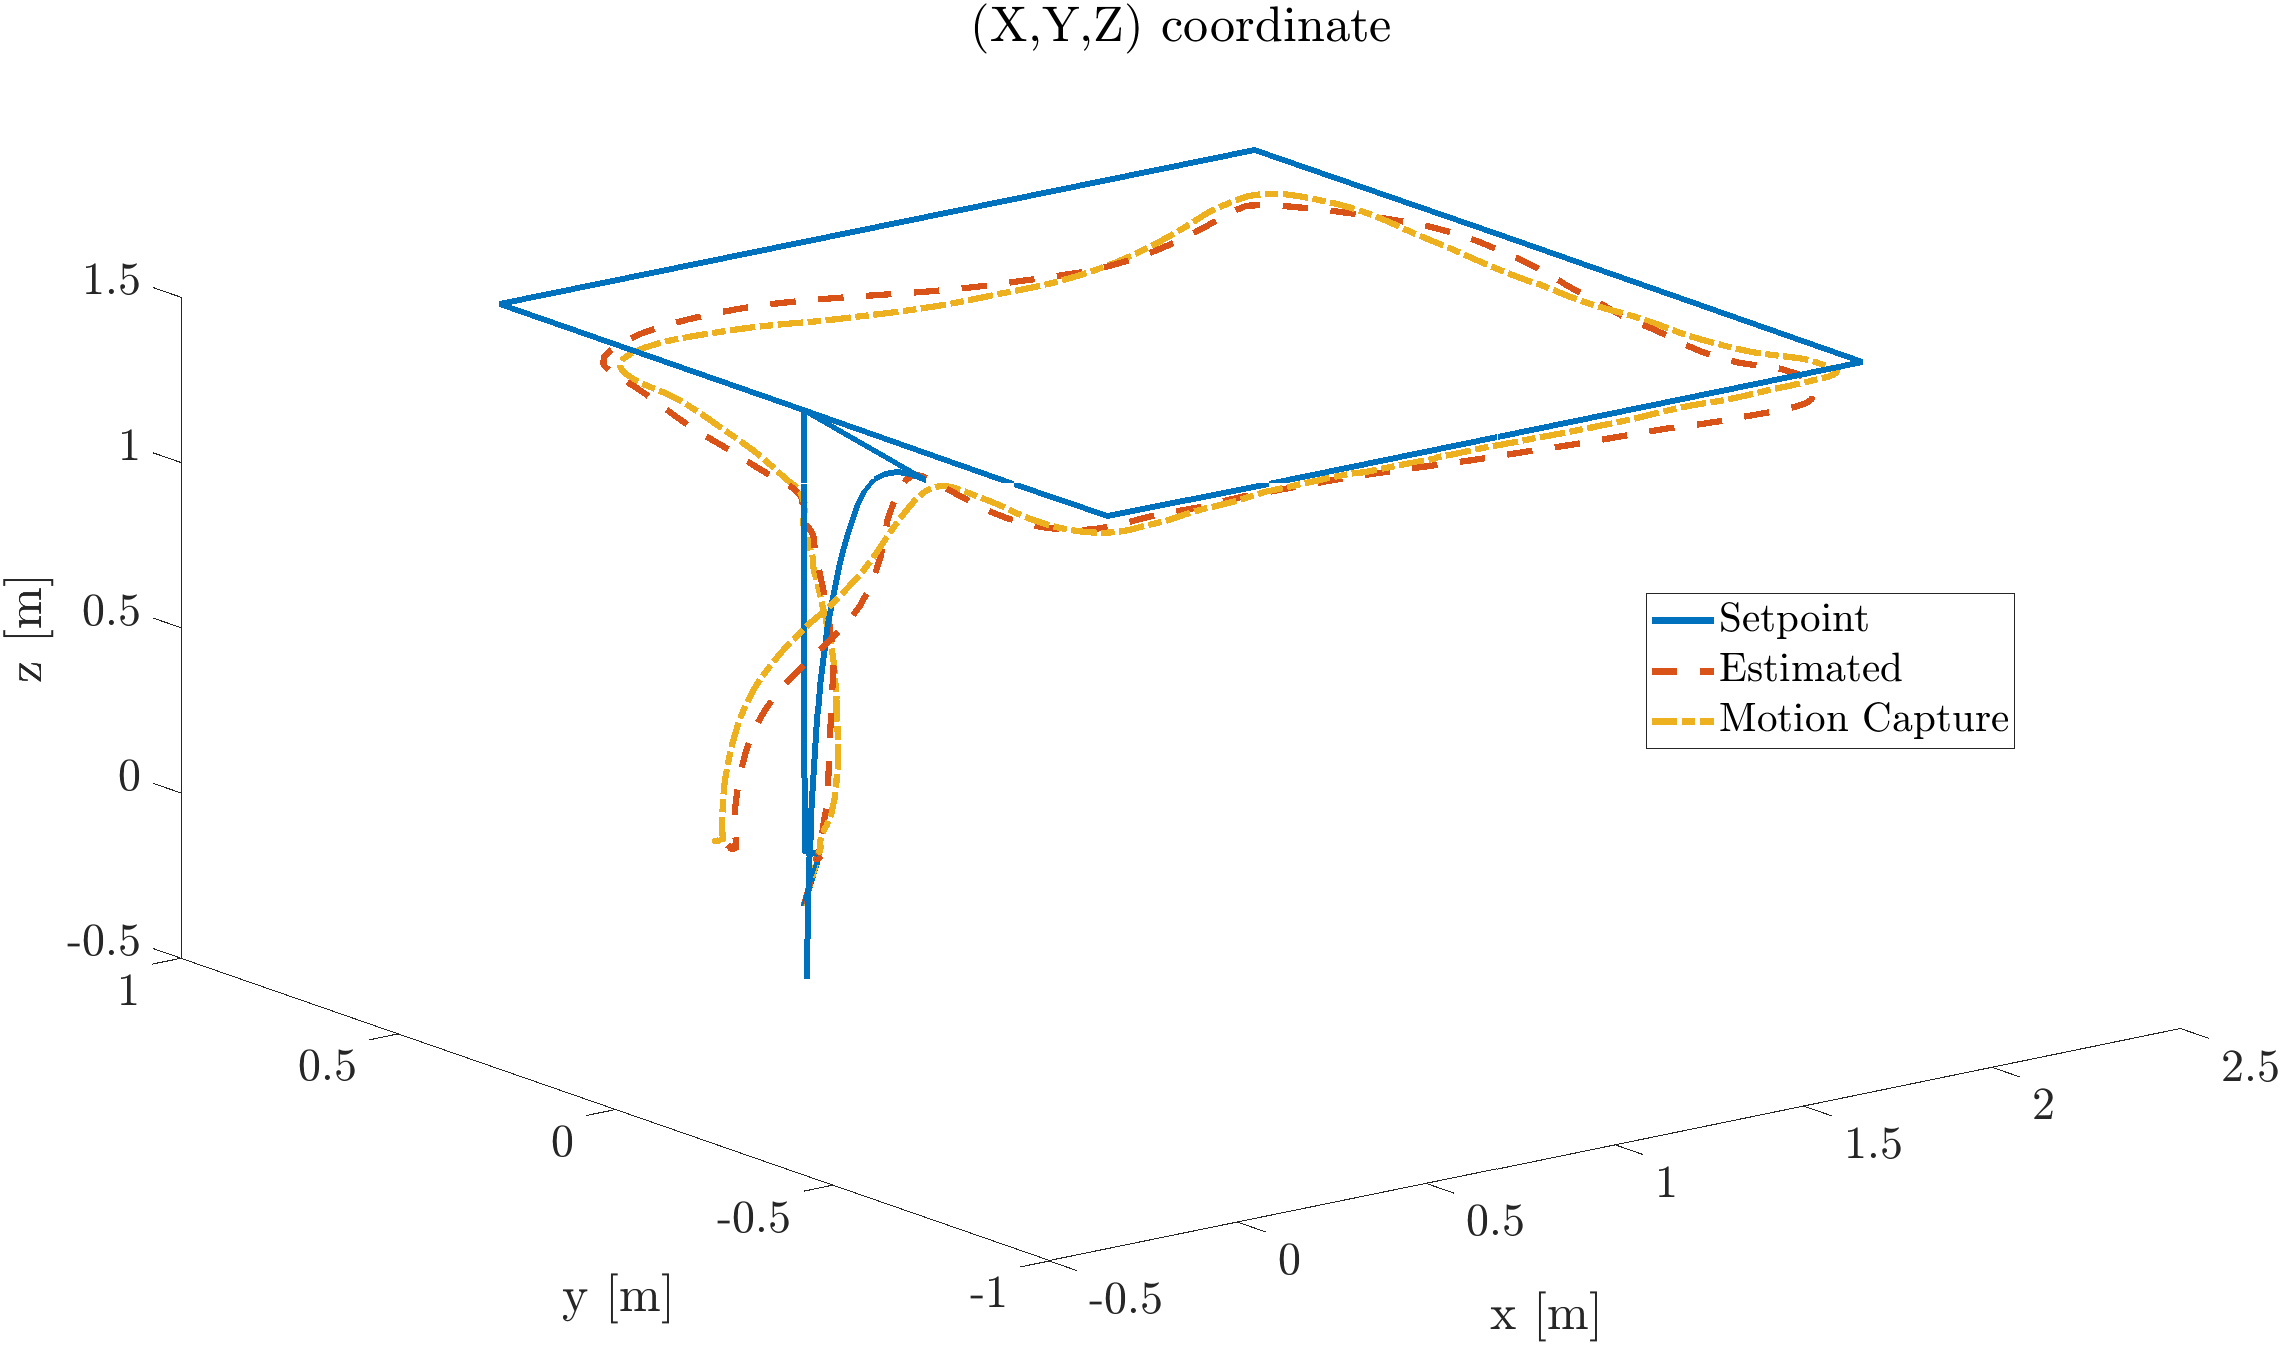
\includegraphics[scale=0.22]{Images/square_trj/xyz_square1.png}
    \caption{Motion capture experimental results}
    \label{fig:mocap_test}
\end{figure}

As can be seen also in Fig. \ref{fig:mocap_test_time}, the estimated trajectory and the MoCap trajectory are more or less the same and they follow quite well the Setpoint trajectory in all three coordinates. This result is what we expected from the Motion capture system which has millimetres accuracy. Therefore the motion capture data will be used as a ground truth for the next tests.  

\begin{figure}
    \centering
    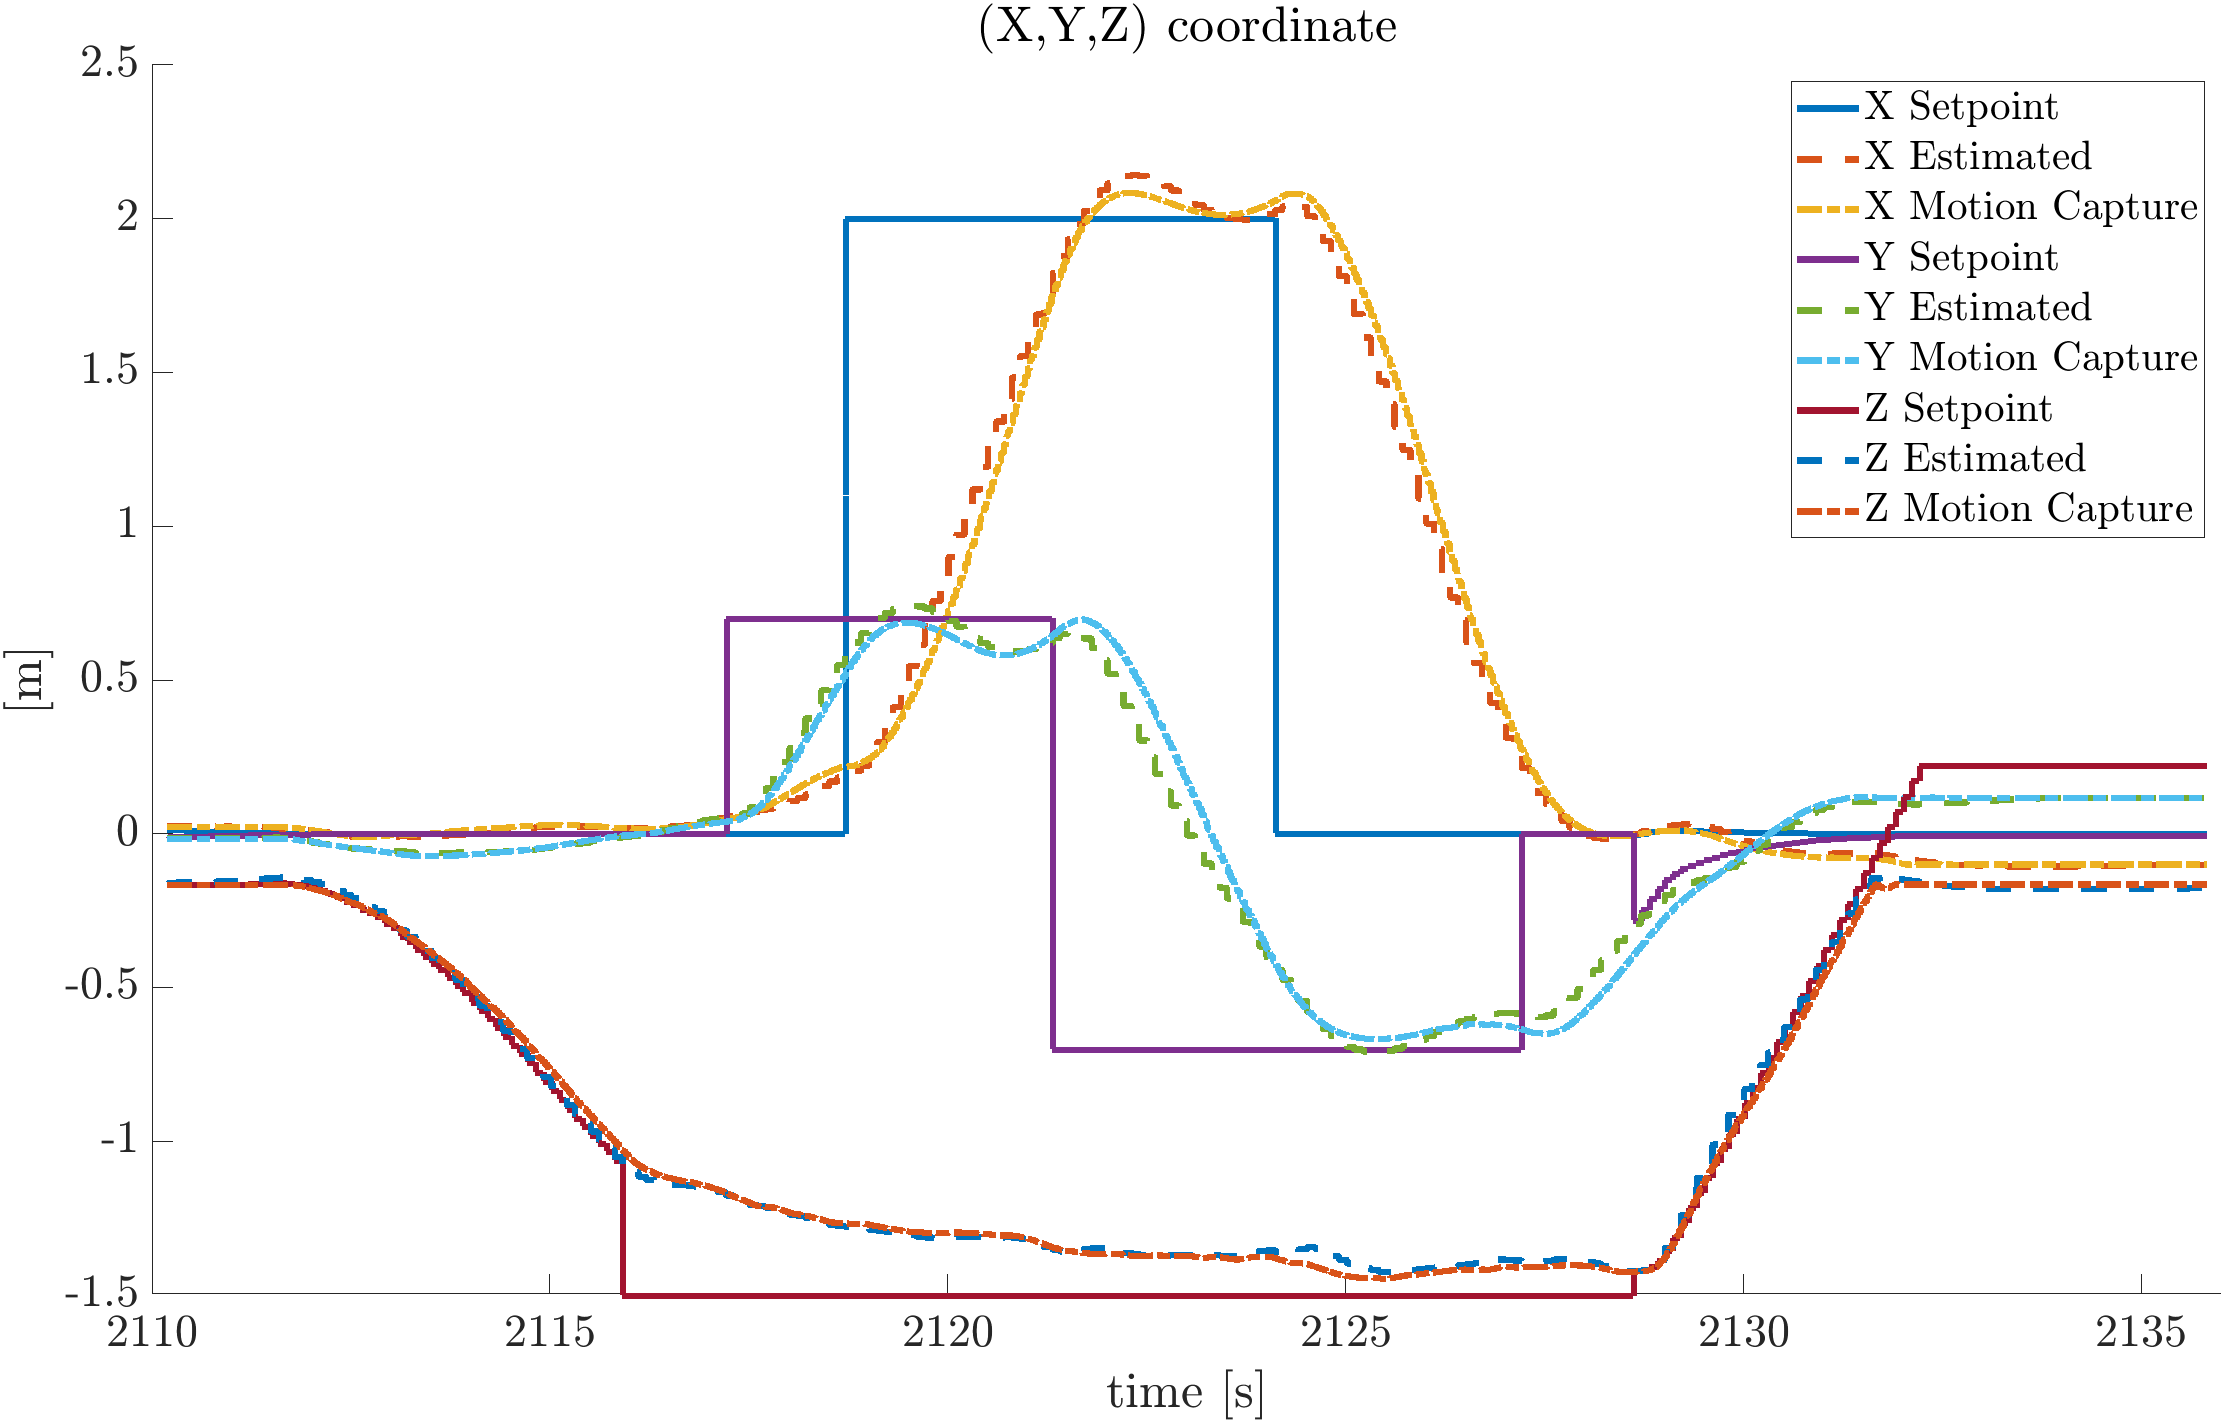
\includegraphics[scale=0.2]{Images/square_trj/xyz_square1_time.png}
    \caption{Motion capture experimental results as a function of time}
    \label{fig:mocap_test_time}
\end{figure}

\subsection{Ultra WideBand and Sonar test results}

The experimental test concerning the Ultra WideBand simulations has been carried out with an infrastructure composed of six anchors, mounted on the top of the MoCap camera, as introduced in the section \ref{Environment-setup}. The drone has been equipped with the UWB tag as described in the section \ref{Drone-setup}.

The UWB infrastructure is shown in Fig. \ref{fig:anchors}, as can be seen, the anchor number 6 is placed in the origin and will be used as the reference one.

\begin{figure}
    \centering
    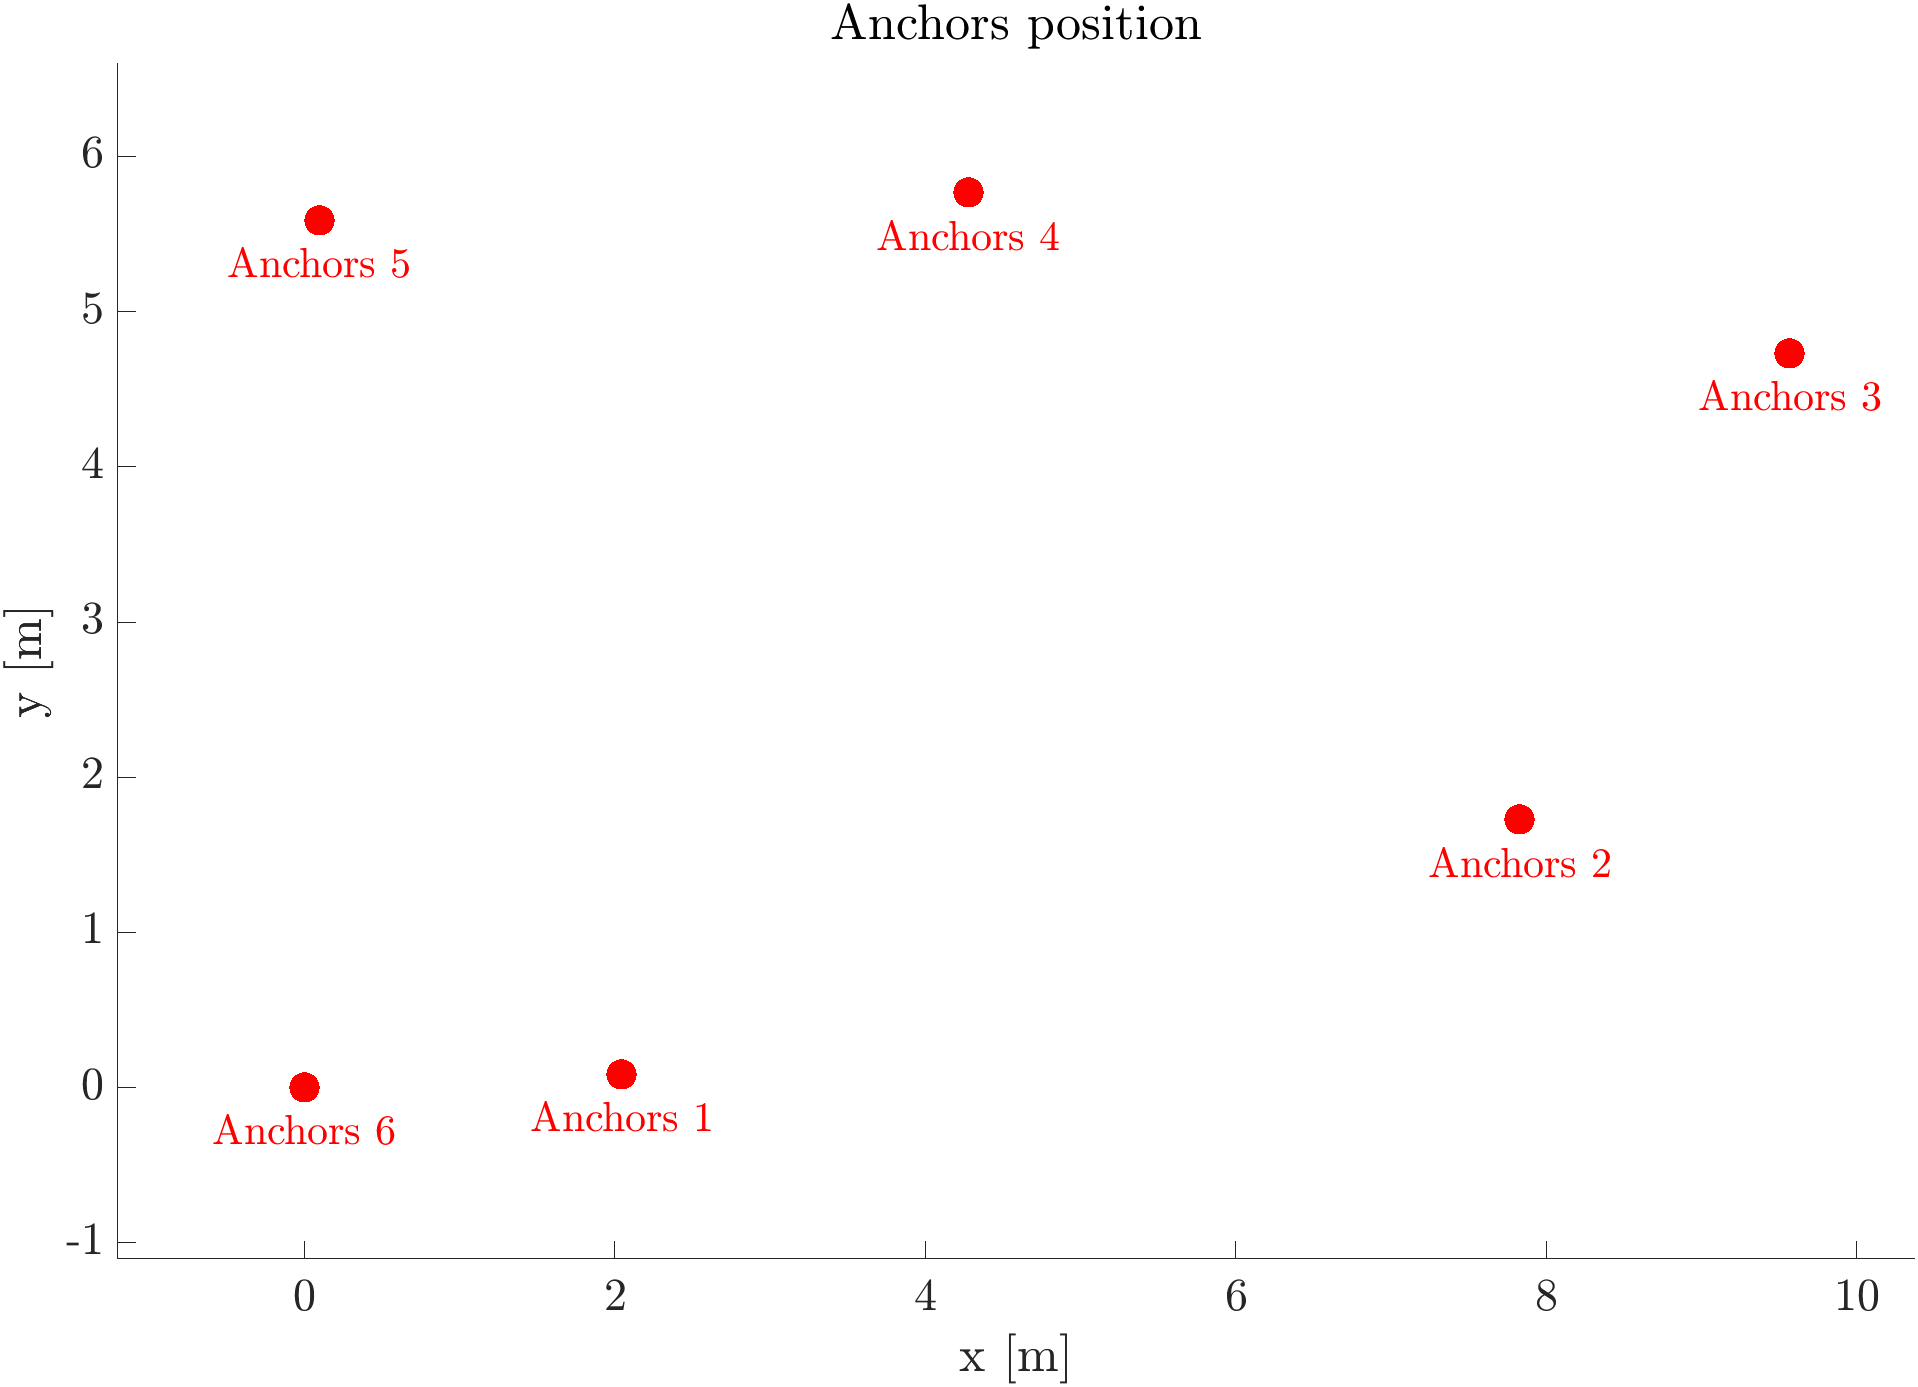
\includegraphics[scale=0.22]{Images/uwb_test/anchors.png}
    \caption{Anchors position}
    \label{fig:anchors}
\end{figure}

To evaluate the UWB test, the position estimated from the UWB system has been compared with the position given by the Motion capture, which has been considered as ground truth. In Fig. \ref{fig:uwb_mocap} the trajectories obtained with UWB and MoCap have been plotted. The UWB position estimate follows the path obtained also in the MoCap position but with poor accuracy which makes it difficult to use the UWB signal to fly. This result is achieved despite the use of an outlier rejection algorithm, which suggests that a stronger outlier rejection is needed with respect to the simulated one.

\begin{figure}
    \centering
    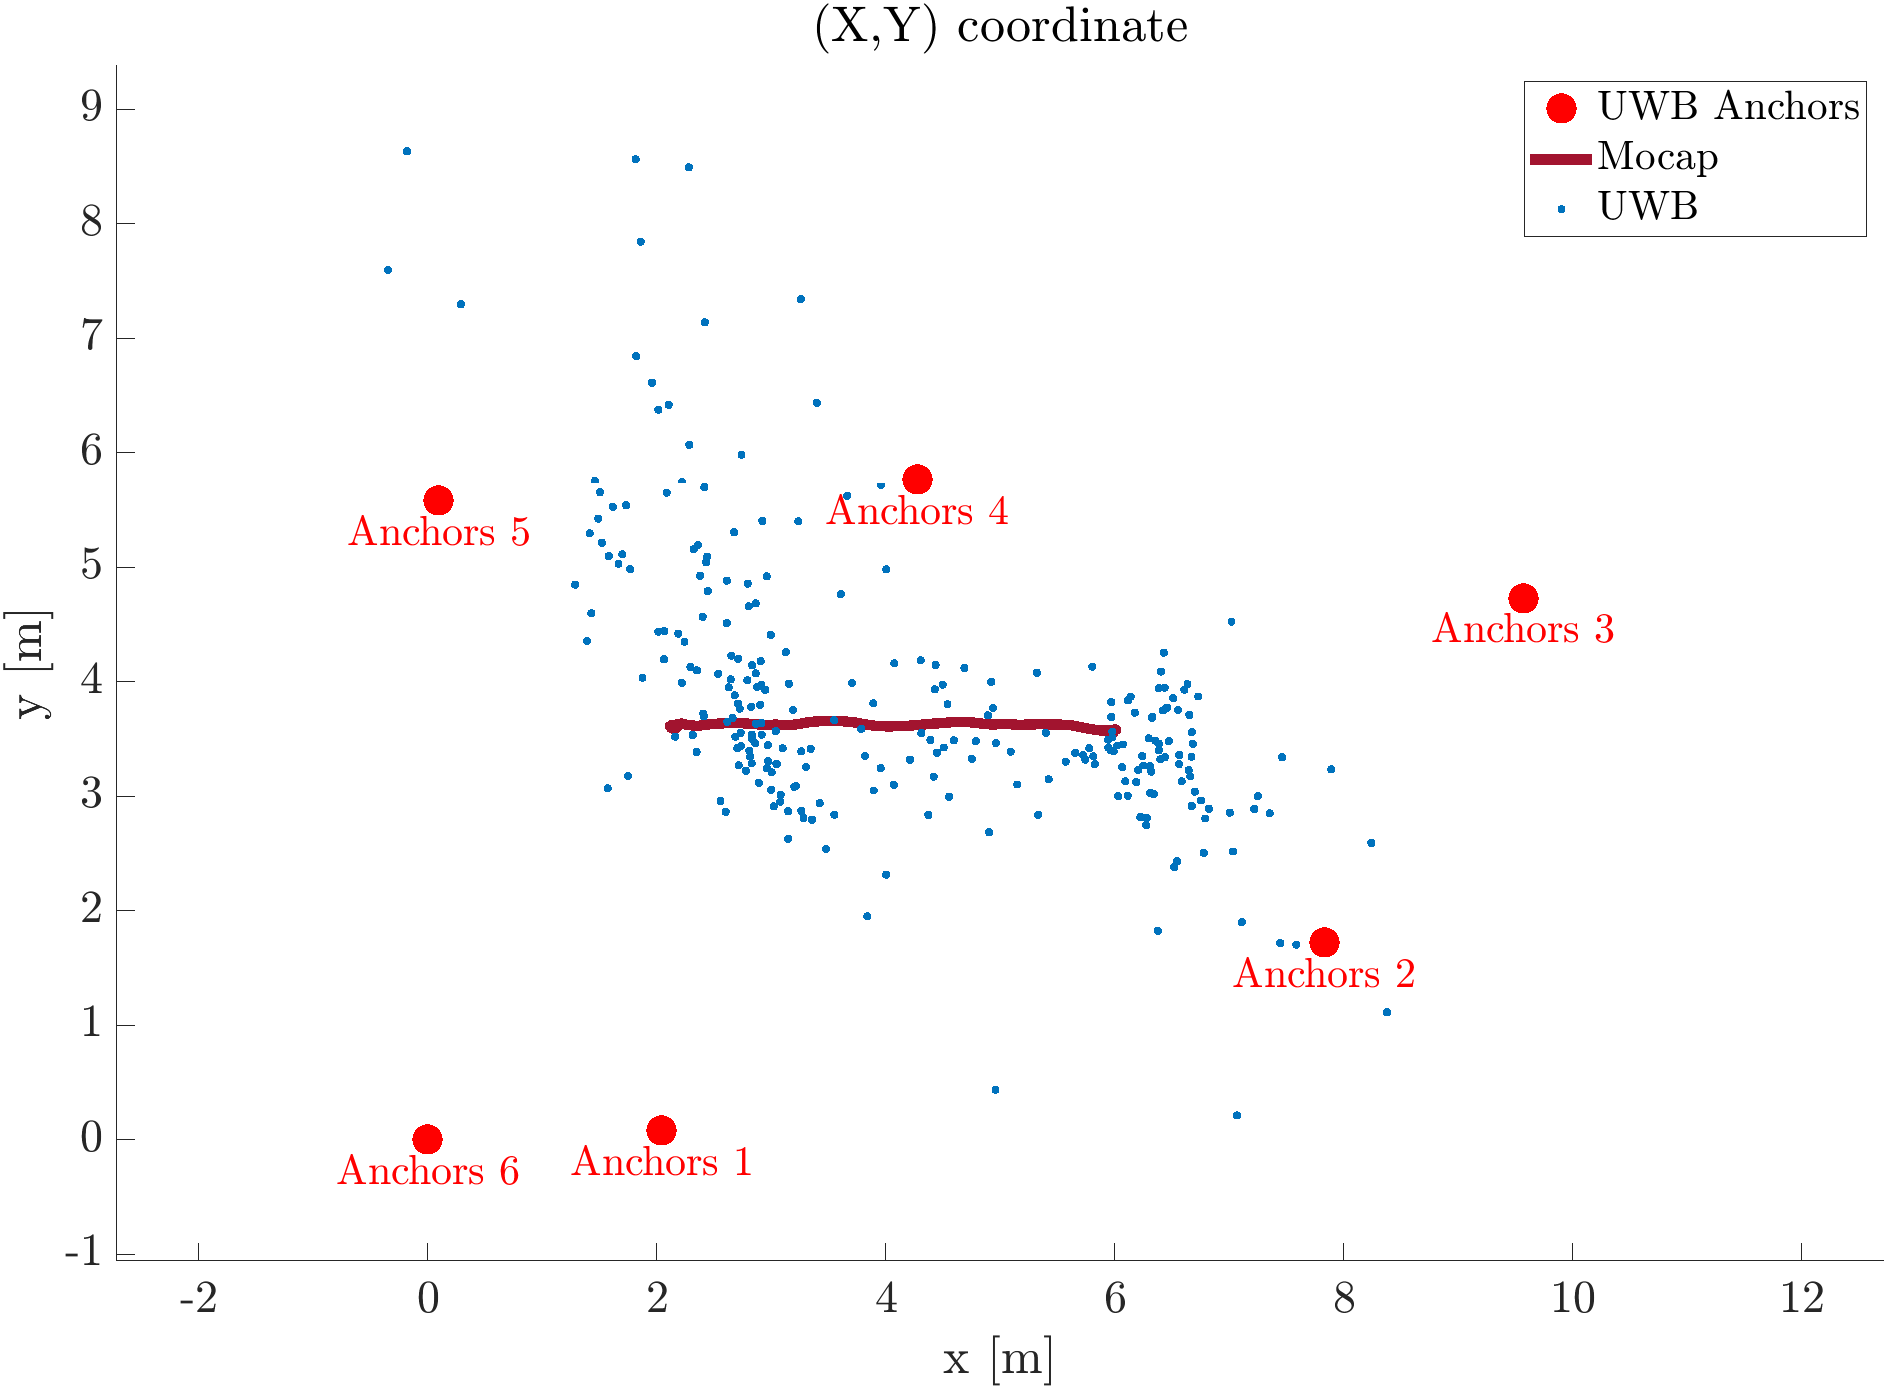
\includegraphics[scale=0.22]{Images/uwb_test/uwb_xy_coordinate.png}
    \caption{UWB and MoCap Trajectory comparison}
    \label{fig:uwb_mocap}
\end{figure}

To better understand the performance of the UWB position estimate has been calculated the error of the UWB signal with respect to the Motion capture signal, using the formula expressed in \ref{eq:err} and plotted the histogram of the error both for the x and y coordinates, Fig. \ref{fig:hist_x} and Fig. \ref{fig:hist_y}.

\begin{equation}
    err_{(x/y)} = (x/y)_{mocap} - (x/y)_{uwb}
    \label{eq:err}
\end{equation}

\begin{figure}
    \centering
    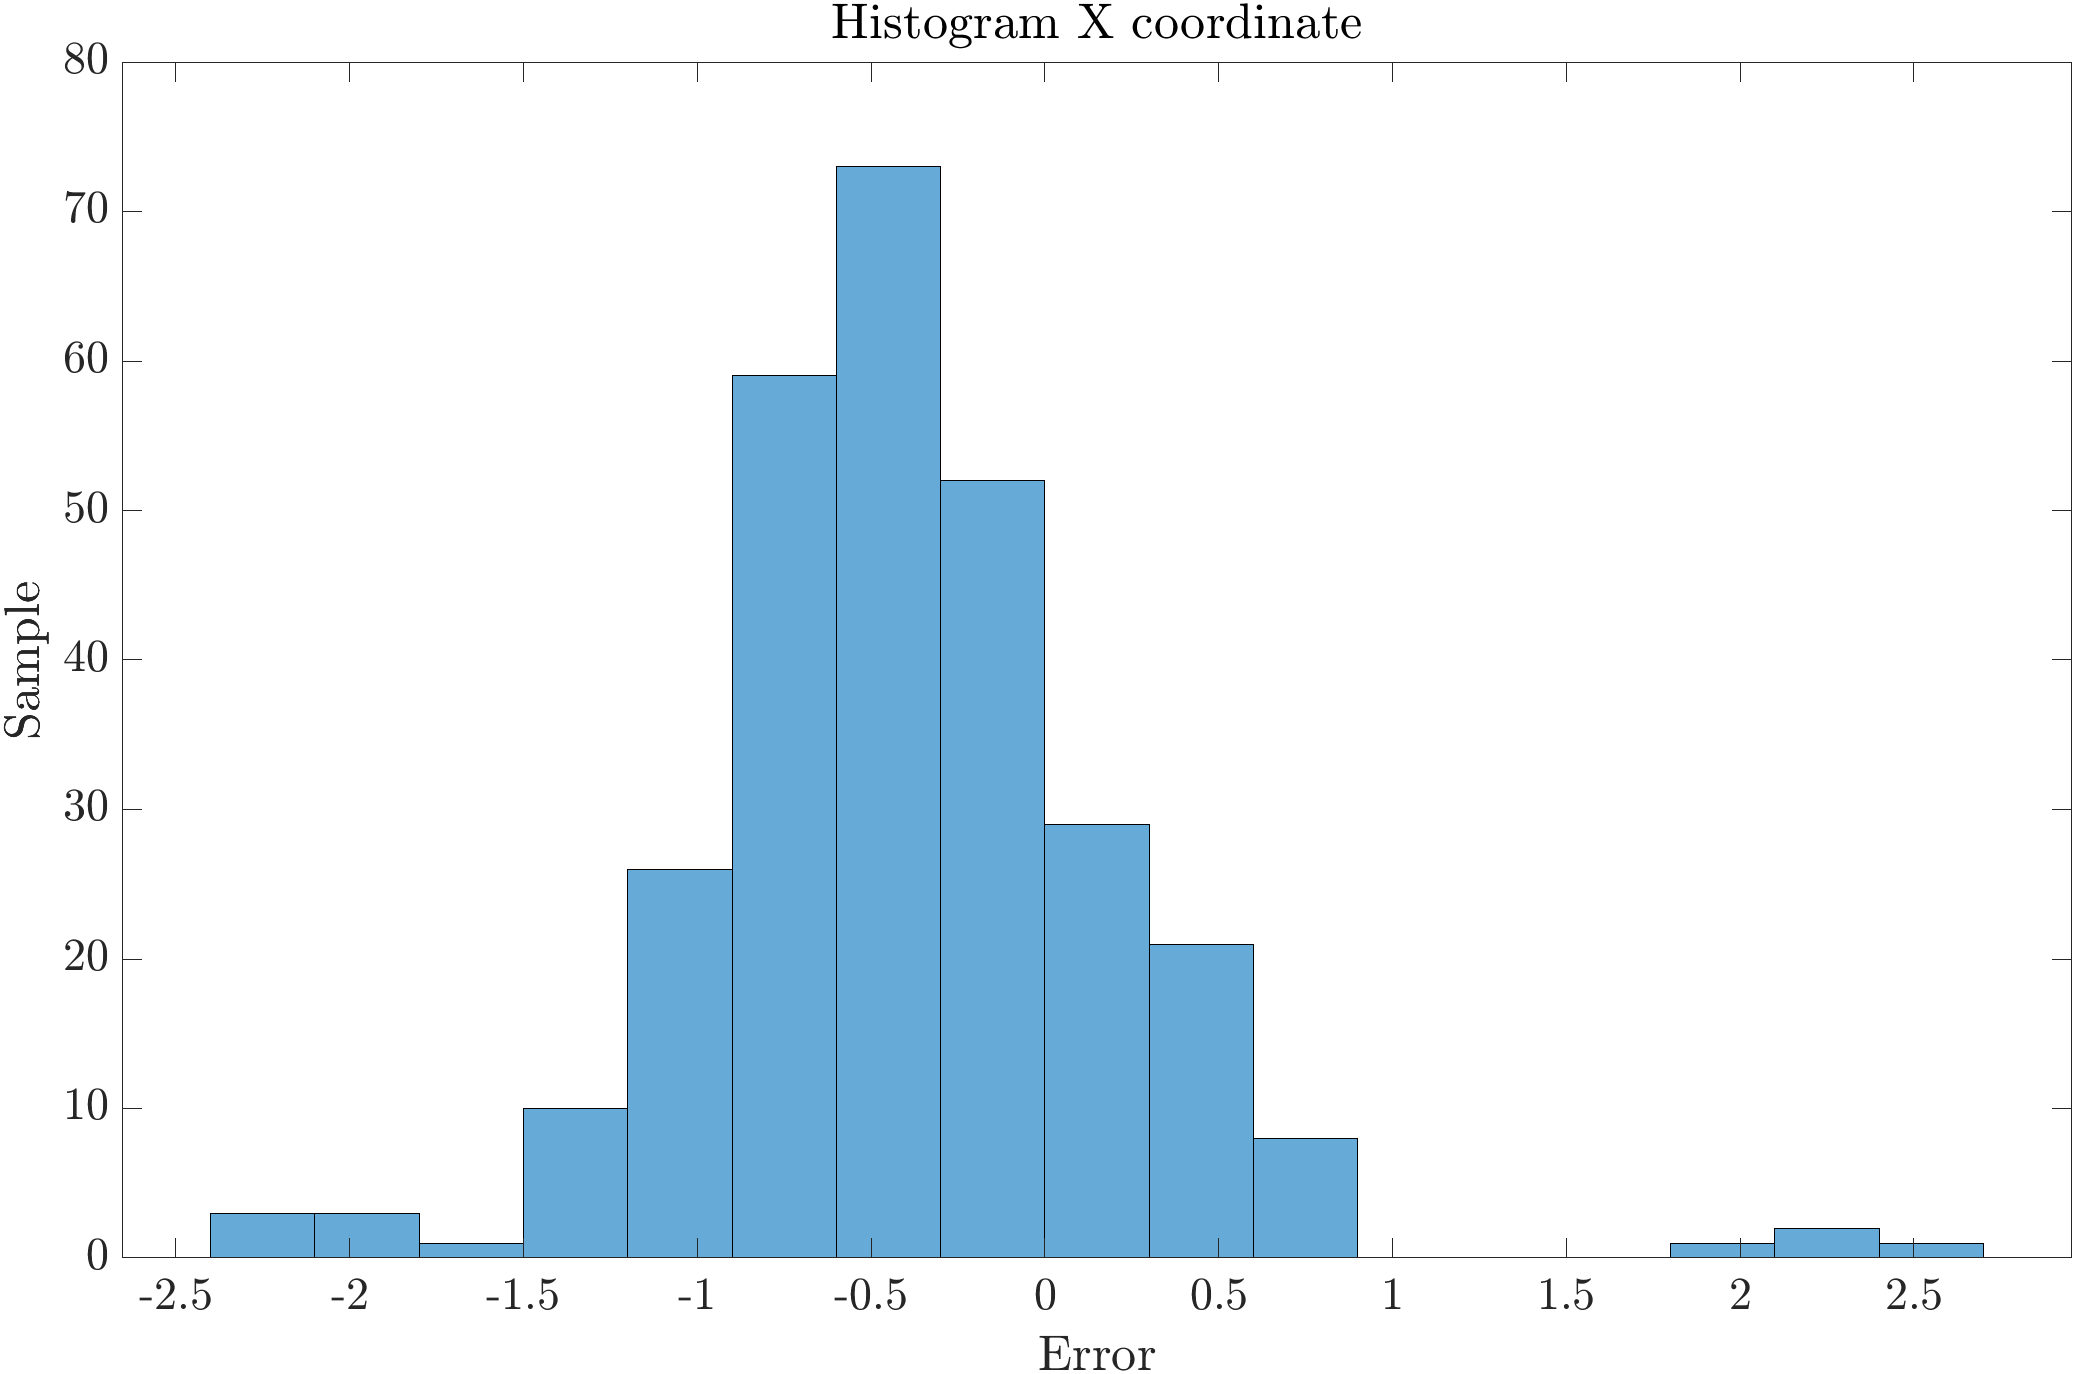
\includegraphics[scale=0.22]{Images/uwb_test/x_hist_uwb.png}
    \caption{Histogram UWB x error}
    \label{fig:hist_x}
\end{figure}

\begin{figure}
    \centering
    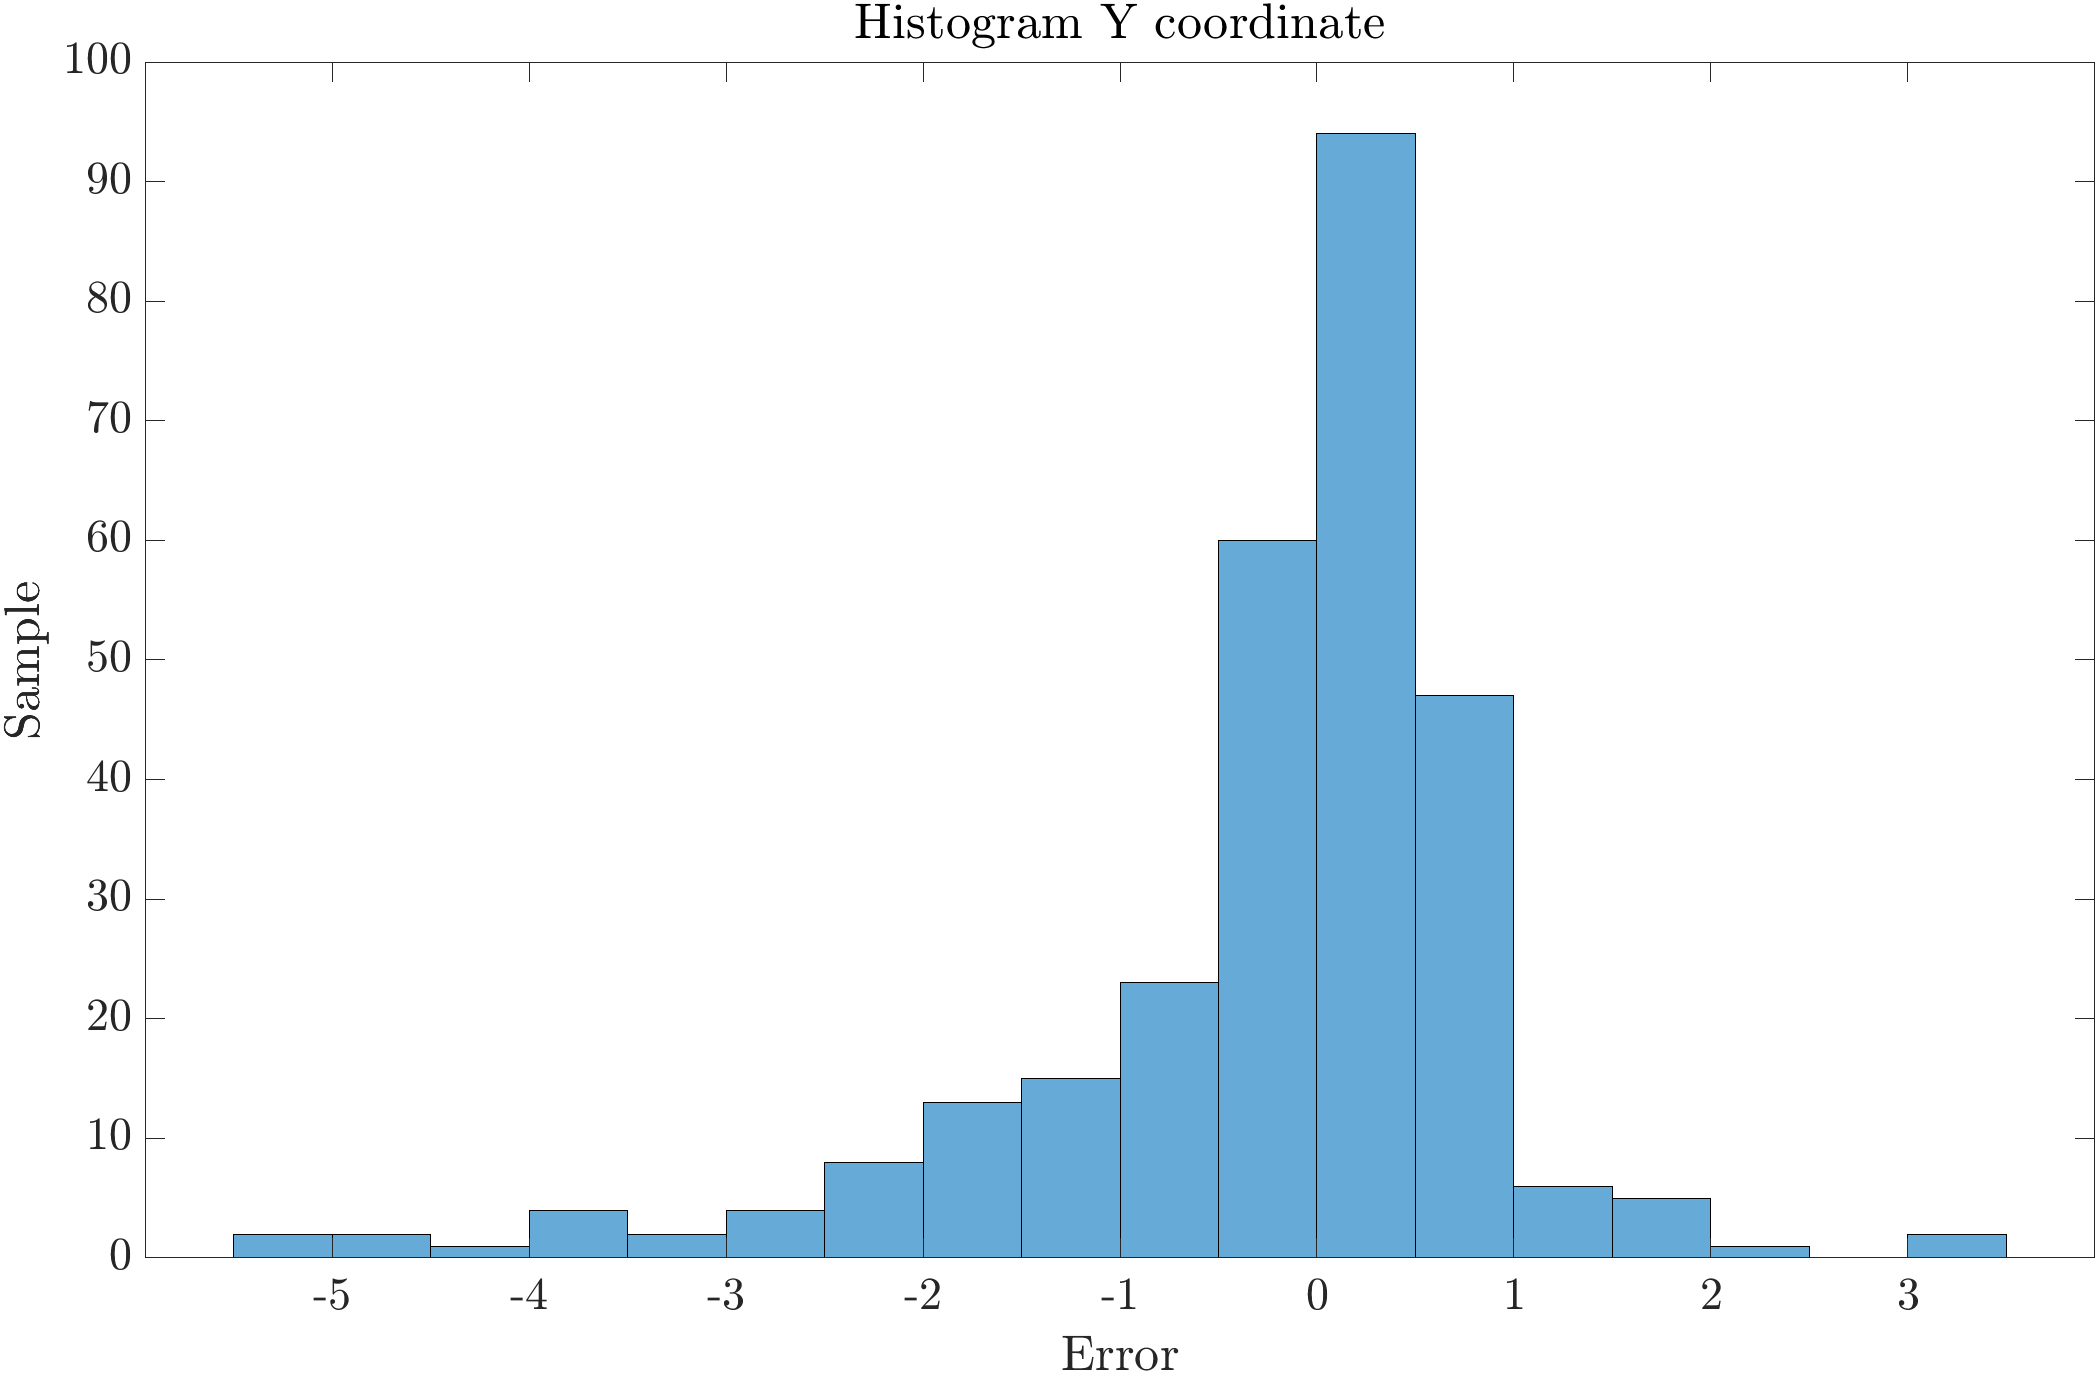
\includegraphics[scale=0.22]{Images/uwb_test/y_hist_uwb.png}
    \caption{Histogram UWB y error}
    \label{fig:hist_y}
\end{figure}

Fig. \ref{fig:hist_x} describes the error committed by the UWB estimating the x coordinate, the histogram shows a Gaussian distribution with mean $\mu_x = -0.38 \ [m]$ and a standard deviation of $\sigma_x = 0.63 \ [m]$.

Fig. \ref{fig:hist_y} instead describes the error committed by the UWB estimating the y coordinate, the histogram shows a Gaussian distribution with mean $\mu_y = -0.24 \ [m]$ and a standard deviation of $\sigma_y = 1.18 \ [m]$.

%% Ultrasonic sensor mb1202
As previously mentioned, since it is not possible to correctly estimate the z coordinate using UWB, the drone was equipped with an ultrasonic sensor on the bottom, in particular the MaxBotix MB1202 one. In order to evaluate the precision of the signal provided by this sensor, the same procedure of the UWB case was adopted, collecting data and comparing them with the Motion Capture coordinate, used as ground truth. In Fig. \ref{fig:mb1202_traj} it is possible to infer that the sensor follows quite well the signal supplied by the MoCap system, as expected. It is important to mention that this result is achieved after a proper outliers rejection, since without filtering the signal it presents some peaks that deviate from the ground truth. The remaining discrepancies between the two signals are outliers that have not been rejected by the algorithm. The initial step in Fig. \ref{fig:mb1202_traj} is due to the fact that the minimum distance that the MB1202 sensor is able to detect is $0.25 \ [m]$: for this reason, the data collected are initially set to zero and they jump to a different value at the first useful measure. The same can be notice at the end, where the MoCap signal reaches zero while the sensor one stabiles to its minimum value. Finally, Fig. \ref{fig:hist_z} describes the error committed by the ultrasonic sensor, computed in the same way as shown above for the UWB case: 

\begin{equation}
    err_z = z_{mocap} - z_{sensor}
\end{equation}

The histogram shows a Gaussian distribution with mean $\mu_z = 0.022$ and standard deviation $\sigma_z = 0.094$. The maximum deviation, which is about $0.25 \ [m]$, is due to the initial and final discrepancies explained above.

\begin{figure}
    \centering
    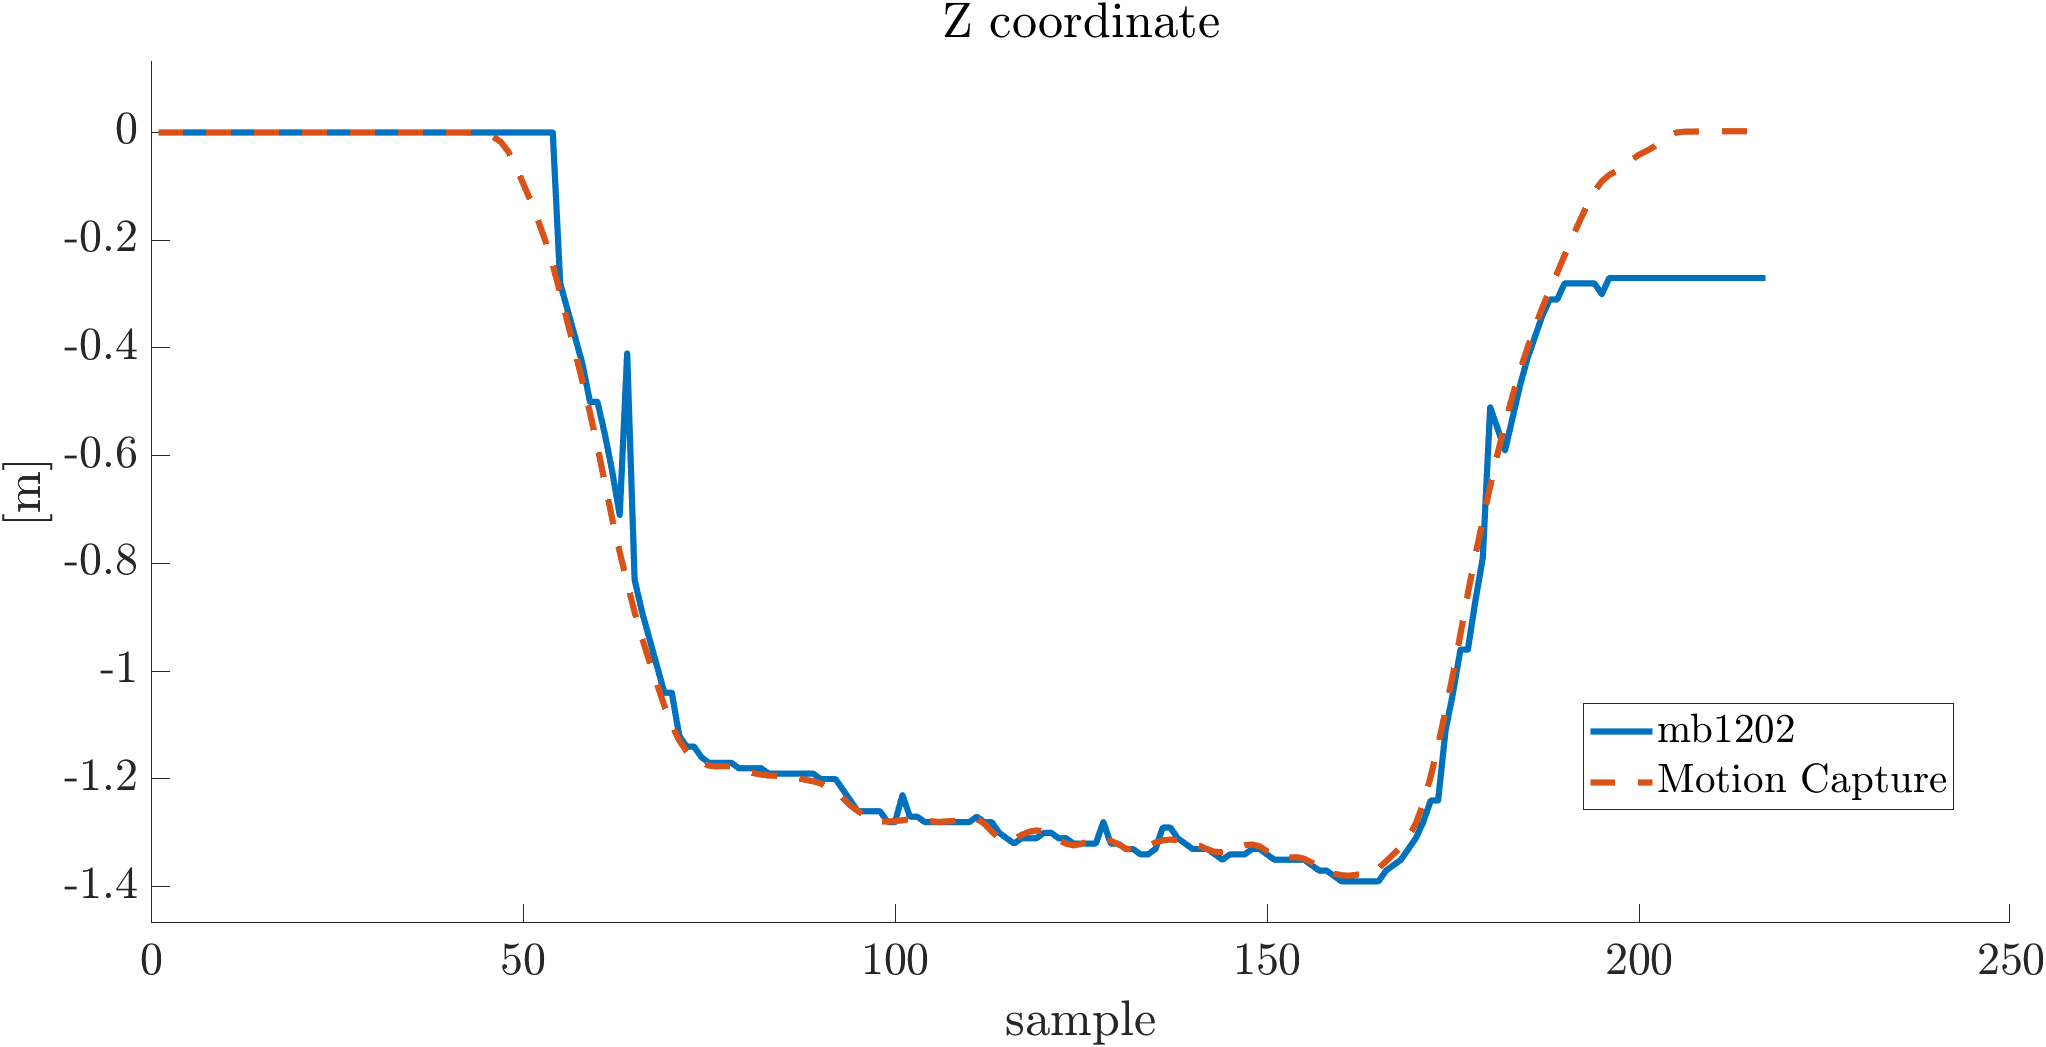
\includegraphics[scale=0.22]{Images/mb1202_filtered.png}
    \caption{Sonar and MoCap trajectory comparison.}
    \label{fig:mb1202_traj}
\end{figure}

\begin{figure}
    \centering
    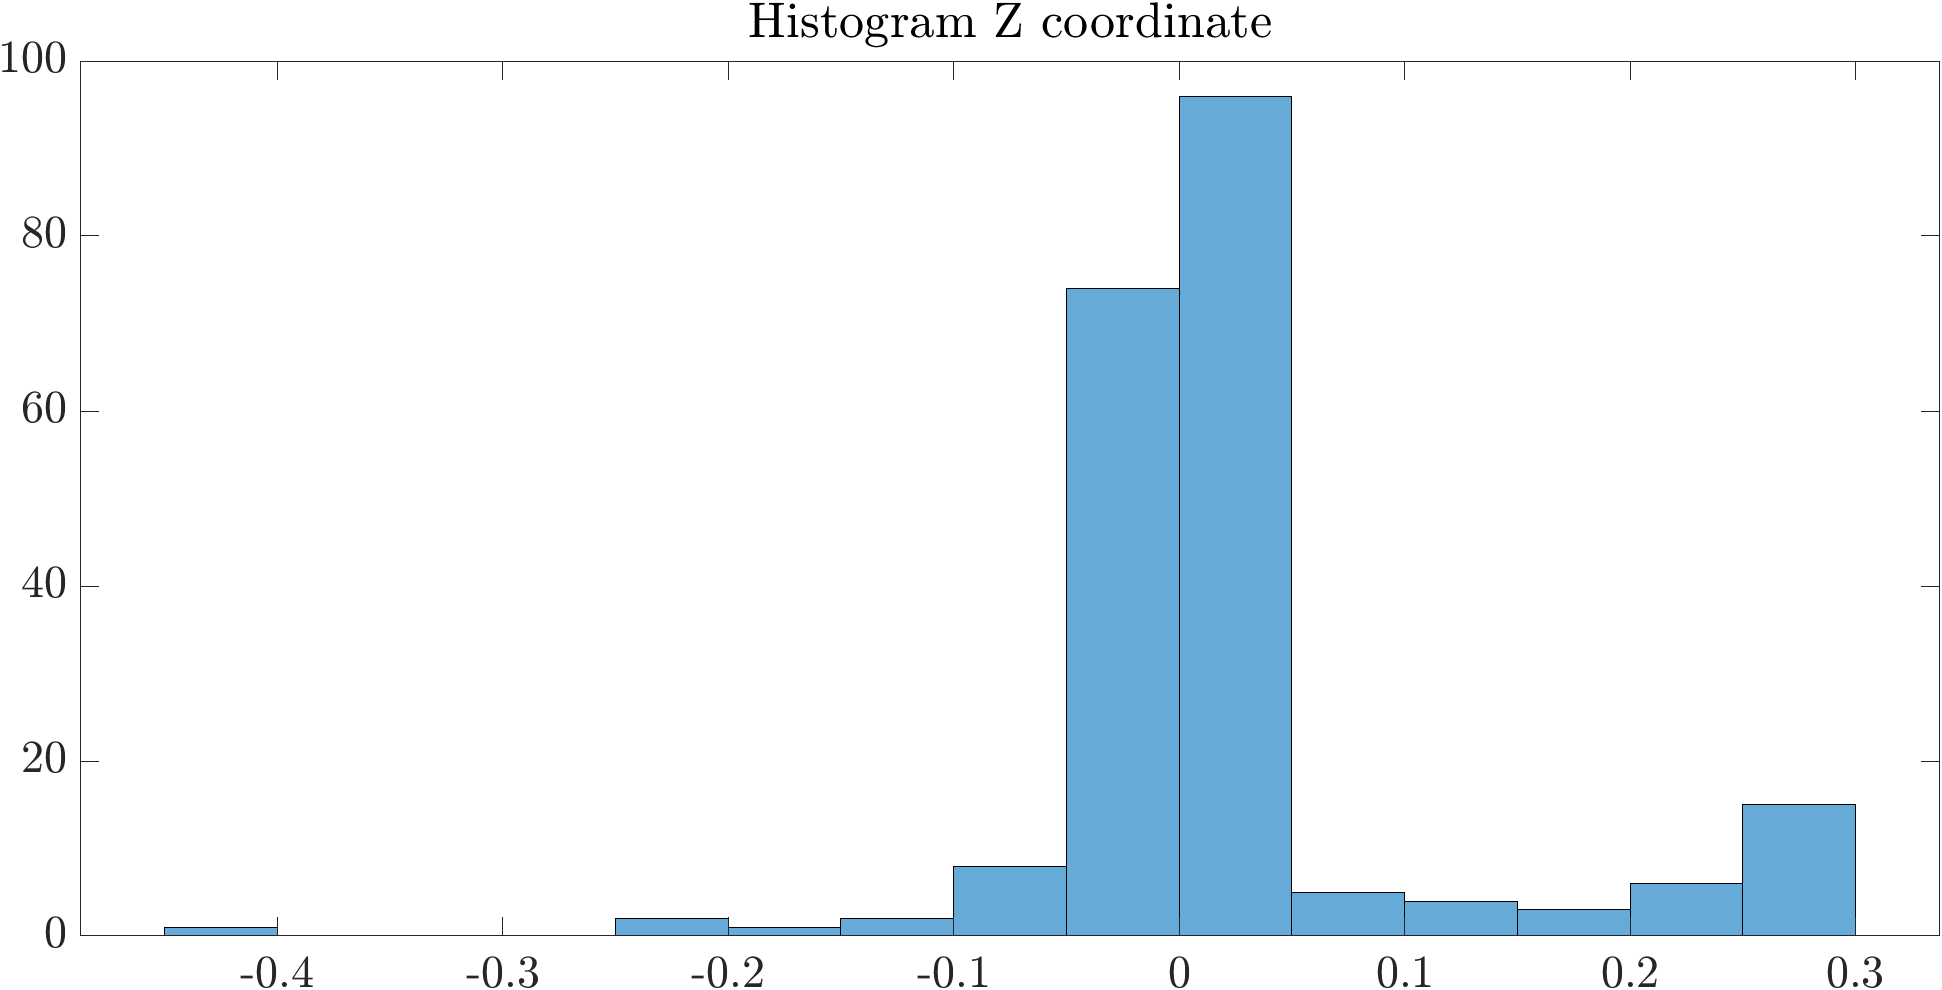
\includegraphics[scale=0.22]{Images/z_hist_mb1202.png}
    \caption{Histogram MB1202 z error.}
    \label{fig:hist_z}
\end{figure}


\section{Conclusions}

Throughout the analysis of different positioning methods presented in this report, it is possible to infer that GPS proved effective but, due to its non-negligible error, makes it more difficult to control the drone in position. Motion Capture performed as expected, showing high precision and reliability. However, the UWB method exhibited considerable error, highlighting the need for enhancement to improve its reliability and precision in positioning. 

Possible future implementations, concerning the GPS method, could explore the integration of Real-Time Kinematics GPS (GPS-RTK) for enhanced outdoor positioning accuracy, addressing the limitations observed in GPS-based methods. Another option is to control the vehicle in velocity instead of position. 
Instead, UWB firstly requires to improve the precision of the infrastructure, since excessive outliers are observed within the data. Simultaneously, an improvement is essential in filtering the signal, refining the outlier rejection algorithm. The current windowing method is significantly impacted by the abundance of outliers, rendering it occasionally ineffective. Strengthening this algorithm is crucial to ensure robust outlier handling and enhance the overall efficacy of the UWB positioning system. Another possible improvement is to apply an Extended Kalman Filter (EKF) before publishing the UWB position, since the other research works presented above achieved great results using this approach.

Finally, Motion Capture has proven to be flawless and reliable. However, its high cost poses challenges for widespread implementation. Thus, prioritising the enhancement of low-cost methods as UWB appears to be a more feasible approach moving forward.

\ifCLASSOPTIONcaptionsoff
  \newpage
\fi

\bibliographystyle{./IEEEtran}
\bibliography{./IEEEabrv,./IEEEexample}

\end{document}